\documentclass[10pt]{article}
\usepackage{kennyworkman}

\newcommand\restr[2]{{% we make the whole thing an ordinary symbol
  \left.\kern-\nulldelimiterspace % automatically resize the bar with \right
  #1 % the function
  \vphantom{\big|} % pretend it's a little taller at normal size
  \right|_{#2} % this is the delimiter
}}

\title{Hatcher: Algebraic Topology}
\author{Kenny Workman}
\date{\today}

\begin{document}

\maketitle

\section{The Fundamental Group}

\subsection{Intuition}

\textbf{The Borromean rings} are three linked circles where any two circles without a third are unlinked. It is a nice object that elucidates the difference between abelian and nonabelian fundamental groups.

Label the three rings $A$, $B$, and $C$. Consider $C$ as an element of $\R^3 \setminus A \cup B$. $C$ can be represented as $aba^{-1}b^{-1}$, where $a$ and $a^{-1}$ are forward and reverse oriented paths around $A$ (and $B$). This element is not trivial, so the free group generated by $a$ and $b$ is not abelian.

Modify the ring so that $A$ and $B$ are linked. The same $C = aba^{-1}b^{-1}$ is now trivial. It is easiest to see this visually. Refer to the picture in Hatcher and slide the first loop $a$ all the way around $A$ until it is hanging over the circle. This loop is clearly contractible.

From this, we conclude there are two ways to tell if two circles are linked:

\begin{itemize}
	\item{Show that one of the circles is an element of the fundamental group of the complement of the other circle. (Simple example of loop wrapping around a circle.)}
	\item{Show the fundamental group of the complement of both of the circles is the abelian. (As in the Borromean ring example.)}
\end{itemize}

\subsection{Basic Constructions}

\begin{definition}[Path]
A path in the space $X$ is a continuous map $f: I \to X$ where $I$ is the unit interval $[0, 1]$.
\end{definition}

\begin{definition}[Homotopy of paths]
A continuous family of maps represented by the continuous map $f: I \times I \to X$ 
\end{definition}

\begin{example}[Linear homotopy]
Consider two paths $f, g$ that share endpoints ($f(0) = g(0) = x_0$ and $f(1) =
g(1) = x_1$). Any such paths are always homotopic by the homotopy 
\[
h_t(s) = (1-t)f(s) + (t)g(s).
\]

% TODO: show continuity with vector argument

\end{example}


\begin{proposition}[homotopy of paths with fixed endpoints is an equivalence relation]
\end{proposition}

\begin{definition}[The product of paths]

	For paths $f, g$ where $f(1) = g(0)$, we can define the product $h = f \cdot g$ as

\[ h(s) = \begin{cases} 
      f(2s) & 0 \leq s \leq 0.5 \\
      g(2s-1) & 0.5 \leq s \leq 1
   \end{cases}
\]

\end{definition}


\begin{proposition}[The fundamental group is in fact a group]
	$\pi_1(X, x_0)$ with respect to the operator $[f]\cdot[g] = [f\cdot g]$ is a group.
\end{proposition}

\begin{definition}[Reparamterization of a path]
	We can precompose any path $f$ with $\phi: I \to I$ such that $f\phi \simeq f$. $f\phi$ is then the reparameterization of $f$.
\end{definition}

\begin{proof}
	To see our operator is well-defined, $[f\cdot g]$ depends only on $[f]$ and $[g]$. In other words, a homotopy exists between paths in $[f\cdot g]$ if and only if it is the composite of homotopies between paths in $[f]$ and $[g]$.

	First, we verify associativity of the operator. Consider $(f \cdot g) \cdot h$. This product composes the composition of $f$ and $g$ with $h$. Visually, $h$ is the first half and $g$ and $f$ occupy the last quarters of the product path. We can construct a piecewise function to change the proportions of these components - "shrink" $h$, keep $g$ the same and "expand" $f$. $[(f \cdot g) \cdot h]\phi \simeq f \cdot (g \cdot h)$ gives us the desired equivalence.

	Second, we check the identity property of the constant map $c$. $f$ can be reparameterized by the piecewise function that speeds it up for the first half of $I$ and holds it constant at $f(1)$ for the second half where $f\phi \simeq f \cdot c$.

	Third, we verify the existence of an inverse for each $[f]$. Define $[\bar{f}]$ where $\bar{f}(s) = f(1-s)$. Then $f\cdot\bar{f}$ is homotopic to the constant path. To see this construct $h_t = f_tg_t$ where $f_t = f$ on $[0, t]$ and $f_t = f(t)$ on $[1-t, 1]$ and $g_t$ is the inverse of this function. As $t$ approaches $1$, $h_t$ has a larger constant region in its image starting from the middle and growing to the endpoints until $h_1(s) = f(0) = g(1)$ is our constant map at timepoint 1.

\end{proof}

\begin{proposition}[The fundamental group is independent of the choice of basepoint up to isomorphism]
	If $f$ is a loop with basepoint $x_1$ and $h$ is a path from $x_0$ to $x_1$. The map $\beta_h: \pi_1(X, x_0) \to \pi_1(X, x_1)$ defined as $\beta_h([f]) = [h \cdot f \cdot \hat{h}]$ is an isomorphism.
\end{proposition}
\begin{proof}
	$\beta_h$ is well-defined. To see this, if $[f] = [f']$ implies that $f$ and $f'$ are homotopic, so certainly $h \cdot f \cdot \bar{h}$ and $h \cdot f' \cdot \bar{h}$ are homotopic and $\beta_h([f]) = \beta([f'])$.
	$\beta_h$ is a homomorphism. $\beta_h([f \cdot g]) = [h \cdot f \cdot g \cdot \bar{h}] = [h \cdot f \cdot \cdot h \cdot \bar{h} \cdot g \cdot \bar{h}] = [h \cdot f \cdot \cdot h] \cdot [\bar{h} \cdot g \cdot \bar{h}] = \beta_h([f]) \cdot = \beta_h([g])$. 
	$\beta_h$ is an isomorphism.

\end{proof}

\begin{definition}
	A space is \textbf{simply connected} if it is path connected and has a trivial fundamental group.
\end{definition}

\begin{definition}{lift}
	Given $f: Y \to X$ and a covering space $p: \tilde{X} \to X$, a lift of $f$ is a map $\tilde{f}: Y \to \tilde{X}$ that
	satisfies $f = p\tilde{f}$.
\end{definition}

We are about to compute the fundamental group of the circle, but will use
general properties of lifts (and covering spaces) to make the proof efficient.

(a) Given a path $f: I \to X$, and a covering space 
$p$, and some $\tilde{x_0} \in p^{-1}(x_0)$, there
exists a unique lifted path $\tilde{f}$ starting at $\tilde{x_0}$.

(b) Given a homotopy of paths in $X$, a covering space $p$, and some
$\tilde{x_0} \in p^{-1}(x_0)$, there exist a unique homotopy of lifted paths in
$\tilde{X}$ starting at $\tilde{x_0}$.

We can see that both of these statements are specific versions of the more
general statement (c), given a $F:Y \times I \to X$ and a $\tilde{F}: Y \times
\{ 0 \} \to \tilde{X}$ lifting $\restr{F}{Y \times \{ 0\}}$, there exists a homotopy
$\tilde{F}: Y \times I \to \tilde{X}$ that lifts $F$ and restricts to the given $\tilde{F}: Y \times \{ 0 \} \to
X$. We'll prove (c) so we can use it later.

\begin{proof}
	We construct a lift of an arbitrary neighborhood $N \times I$.

	Consider a fixed $\{y\} \times I$ and notice that for each
	point $(y, t)$,  $F((y, t))$ lies in some evenly covered open set
	$U_t$.

	Because $F$ is continuous, we can construct an open neighborhood $N_t
	\times (a_t, b_t)$ of $y$ where $F(N_t \times (a_t, b_t)) \subseteq U_t$.

	$\{ N_t \times (a_t, b_t) \}_t$ cover $\{y\} \times I$. Since $I$ is compact,
	we can recover a finite subcollection. Let $N$ be the intersection of all the $N_t$ in
	this subcollection and partition $I$ into $\{ [0, t_1] \cdots [t_i, t_{i+1}]
	\cdots [t_m, 1] \}$ in such a way where each closed interval lies within an
	open set in our subcollection. This partition need not be finite and probably
	is not if all of these closed intervals must lie entirely within the
	previously defined open sets.

	Then $N \times [t_i, t_{i+1}]$ each contain $(y, t)$ for some $t \in [t_i,
	t_\{i+1\}]$, and fixed $y$, while $F(N \times [t_i, t_{i+1}]) \subseteq U_i$,
	an evenly covered open set. Because each $U_i$ is homeomomorphic with some
	sheet $\tilde{U}_i$ by $p$, Starting with $N \times [0, t_1]$, while we are
	only given $\tilde{F}$ for $N \times \{0\}$, we can extend the map to the rest of
	this neighborhood by $Fp^{-1}$ for $p$ defined over the sheet that contains
	$\tilde{F}(N \times \{0\})$. We proceed by induction, defining $\tilde{F}$
	over $N \times [t_i, t_{i+1}]$ using $Fp^{-1}$ over the same sheet
	$\tilde{U_i}$ ($t_i$ is shared by the last neighborhood and all neighborhoods
	must lie entirely in some sheet, so they both lie in the same sheet). The
	only additional adjustment might be restricting $N$ for $N \times [t_i,
	t_{i+1}]$ because it was only restricted sufficiently to lie within some
	$U_i$, but not the one homemomorphic to the sheet that we need (?).

\end{proof}

To see that (c) implies (a), consider a path as a homotopy of points. To see
the same with (b), if we are given a homotopy of paths and the starting point
of their lifted paths, the full lifted paths are uniquely determined by (a). If
we consider $Y$ as $I$, a homotopy of the lifted paths follows.

\begin{theorem}[$\Z \cong \pi_1(S^1)$]

	The fundamental group of $S^1$ is the infinite cylical group generated by the
	loop $\omega(s) = (\cos 2\pi s, \sin 2 \pi s)$
\end{theorem}

\begin{proof}

	First recognize that because $[\omega_n] = [\omega]^n$, where $\omega_n = z
	\mapsto (\cos 2\pi nz, \sin 2\pi nz)$, our proof is
	equivalent to showing any loop $f$ is homotopic to some $[\omega_n]$ because
	it is then a product of our generator.

	Let $p: \R \to S^1$ be a covering space defined as $p = s \mapsto (\cos 2\pi
	s, \sin 2\pi s)$. We will first state two useful properties of lifts with
	this covering space and use these to show our result without proof before
	proving them.

\end{proof}

We can immediately use $\pi_1(S^1)$ to prove important theorems. The big idea is that each full rotation around the circle is a unique element of the group. This suggests, among other things, that a loop once around cannot be continuously deformed to a loop twice around.

Our arguments proceed by contradiction, by assuming that our desired result does not hold and showing that this assumption implies some homotopy between loops on the circle that is not allowed.

\begin{theorem}[Fundamental Theorem of Algebra]
Every non constant polynomial with coefficients in $\C$ has at least one root in $\C$.
\end{theorem}

\begin{proof}
	Assume our polynomial $p(z) = z^n + a_1z^{n-1} ... a_n$ has no roots.
	Define the following $f_r: I \to \C$ for each real number:
	\[
		f_r(s) = \frac{p(re^{2\pi is}) \backslash p(r)}{\abs{p(re^{2\pi is})} \backslash \abs{p(r)}}
	\]
	We claim this is a loop in the unit circle $S^1$. To see this, compute some values for fixed $r$ and note for any value of $r$, $f_r(0) = 1$, $f_r(1) = 1$.
	Note that $f_0$ is a constant map with value $1$ and is the trivial loop. Then by varying $r$ we obtain a homotopy between any $f_r$ and $0$ with (the embedded) basepoint $(1, 0)$.
	\indent We now show that $p$ must be constant. Choose a large $r$ such that $r \geq \sum_n{\abs{a_n}} \geq 1$. Observe then $r^n = rr^{n-1} \geq (\sum_n{\abs{a_n}})r^{n-1}$.
	This expression motivates a new homotopy for each $f_r$, let $f_{(r, t)}$ be our previous definition with $p_t(z, t) = z^n + t(z^{n-1}a_1 + ... a_n)$ substituted for each $p$. See that $f_t$ has no zeros on the circle of complex values with radius $r$ satisfying our expression (this is why we constructed it at all).
	Note that $f_{(r, 0)} = e^{2\pi stn}$ (check). Then $f_{(r, t)}$ is a homotopy between $f_r$ and homotopy class $[w_n] \in \pi_1(S^1)$.  But $f_r$ is homotopic to $0$. Then $w_n$ is also homotopic to $0$ and $n$ must be 0. Our $p(z) = a_n$ must be constant.
\end{proof}

\begin{theorem}[Brouwer fixed point theorem]
	Any continuous map $h: D^2 \to D^2$ must have a fixed point $h(x) = x$.
\end{theorem}

This theorem was initially proved by a gentleman named L.E.J. Brouwer circa 1910 and seems to be foundational to the rest of algebraic topology and other fields like differential topology.

We now introduce a theorem which proves that there must exist two antipodal
locations on the surface of the earth with the same temperature and pressure
(assuming that temperature and pressure are continuous functions of location).

\begin{theorem}[Borsuk-Ulam theorem]
	A continuous map $f: S^2 \to \R^2$ must have at least one pair of antipodal points $x$ and $-x$ where $f(x) = f(-x)$.
\end{theorem}

Lets build intuition for the two dimensional case by proving the theorem in one
dimensions. For a map $f: S^1 \to \R$, construct continuous $h = f(x) - f(-x)$.
Pick a point $x$, and evaluate $h$ at points $x$ and $-x$ halfway across the
circle from each other. Notice $h(x) = -h(x)$ so there must exist some $y$
where $h(y) = 0 \in [h(x), -h(x)]$ by intermediate value theorem. We proceed
with proof in two dimensions:

\begin{proof}

	Define a path $\eta(s) = (\cos 2\pi s, \sin 2\pi s, 0)$ around the equator of
	$S^2$ and a map $g: S^2 \to S^1$ defined as $g(x) = \frac{f(x) -
	f(-x)}{\abs{f(x) - f(-x)}}$. Let $h = g\eta$. Check that $\eta$ is
	nullhomotopic (one can shrink the equator to one of the poles) and therefore
	$h$ is also nullhomotopic. (If $\eta \simeq 1$ by $\psi: I \times I \to S^2$,
	then $g\eta \simeq g 1$ by $g \psi : I \times I \to S^1$)

	See that because $g(-x) = -g(x)$ and $\eta(s + \frac 1 2) = -\eta(s)$,
	$g\eta(s + \frac 1 2) = g(-\eta(s)) = -g\eta(s)$, so $h(s + \frac 1 2) =
	-h(s)$. We now examine the lift $\tilde{h}$, induced by $p = s \mapsto (\cos
	2\pi s, \sin 2\pi s)$, and see that $\tilde{h}(s+\frac 1 2) = \tilde{h}(s) +x$
	where $x$ are all the values that map $\tilde{h}(s) +x$ opposite to
	$\tilde{h}(s+\frac 1 2)$ under the trigonometric functions composing $p$.
	Then $x = \frac q 2$ where $q$ is an odd integer. (Check this. Hatcher skips
	some steps that most readers would find obvious probably).

	Think about what we are doing here - lifting $h$ from its path on $S^1$ to
	$\R$ - stretching it out "flat" so we can see how much it winds along $S^1$.

	If $\tilde{h}(s + 1/2) = \tilde{h}(s) + \frac q 2$, we can solve for $q$, $q
	= 2(\tilde{h}(s + 1/2) - \tilde{h}(s))$, and see it cannot be a continuous
	function of $s$ unless it is constant because it is constrained to integer
	values. Then $\tilde{h}(1) = \tilde{h}(\frac 1 2) + \frac q 2 = \tilde{h}(0)
	+ q$, so $\tilde{h}$ is a path that travels a distance $q$ on $\R$, so must wind
	around $S^1$ $q$ times (is $q$ times a generator in $S^1$). So $h$ is not
	nullhomotopic because $q$ is not 0.

	But we saw that $h$, as the composition $g \cdot \eta$, is nullhomotopic.
	This is a contradiction.

\end{proof}

% TODO, really see the role of Borsuk Ulam in the above proof

Reflecting on the structure of this proof for a moment, it is the existence of
some continuous map $g: S^2 \to S^1$. Intuition tells us that the nullhomotopy
sliding the equator to a pole should do nothing when embedded in $S^1$

This theorem says a few things. It tells us the surface of a sphere can never
be one-to-one with an embedding in $R^2$, as two of the points always collapse,
so it cannot be homeomorphic with a subspace of $R^2$. This is obvious when you
think of the stereographic projection of the sphere onto the plane, but is hard
to prove in general.

\begin{exercise}[8]
	Does the Borsuk-Ulam Theorem hold for the torus? For some continuous $f: S^1
	\times S^1 \to \R^2$, does there always exist $(x, y)$ and $(-x, -y)$ where $f((x, y)) = f((-x, -y))$.
\end{exercise}

\begin{figure}[ht!]
\centering
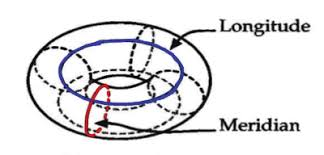
\includegraphics[width=90mm]{meridian-longitude-torus.jpeg}
\caption{A refresher on the meridian and longitude of the torus.}
\end{figure}

\begin{proof}
	We can't do the exact same thing as the proof for $S^2$ because loops on the surface of the
	torus are not nullhomotopic.

	Consider the stereographic projection $p$ of the torus resting on the $0XY$
	plane to this plane. This map is continuous. Each point, denoted $(x, y) \in
	S^1 \times S^1$ on the torus that share an image on the plane must lie on the same meridian
	circle, so must share the first coordinate. Then there cannot be antipodal points
	that satisfy $p((x, y)) = p((-x, -y))$. ($x = 0$ does not lie on $S^1$).
\end{proof}

\begin{note}[Explicit parameterization of torus]
The above problem is mostly an exercise in visualizing geometry and explicit
equations are useful to understand the shape under study.

For $0 \leq \theta \leq 2\pi, 0 \leq \phi \leq 2\pi$ and $r, R$ constants
(the radius of the meridian tube and distance from origin to center of the
meridian tube respectively)
\[z = r \sin \theta \]
\[y = (R + r \cos \theta) \sin \phi \]
\[x = (R + r \cos \theta) \cos \phi \]

See the below figure.

Then continuous $(x, y, z) \mapsto (x, y)$, always maps $(x, y, z)$ and $(-x,
-y, z)$ to different points.
\end{note}

\begin{figure}[ht!]
\centering
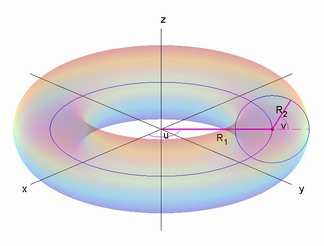
\includegraphics[width=90mm]{torus_parameterization.jpg}
\caption{Illustration of paramterization of torus}
\end{figure}


\begin{theorem}[Fundamental group of a product space]
	$\pi_1(X \times Y) \cong \pi_1(X) \times \pi_1(Y)$ if $X$ and $Y$ are path connected.
\end{theorem}

\begin{proof}
	Recall a map into a product space $f: Z \to X \times Y$ is continuous iff
	constituent maps $g: Z \to X$ and $h: Z \to Y$ are continuous. Then each loop
	$\omega: I \to X \times Y$ has equivalent pairs of loops $\omega_X: I \to X$
	and $\omega_Y: I \to Y$. Similarly, homotopies of loops the product space
	have equivalent homotopies in the constituent spaces, which we can use to
	show that $\phi: \pi_1(X, Y) \to \pi_1(X) \times \pi_1(Y)$ defined as $[f]
	\mapsto ([g], [h])$ is a group homomorphism.
\end{proof}

\begin{exercise}[1.1.10]
	From the isomorphism $\pi_1(X \times Y, (x_0, y_0)) \cong \pi_1(X, x_0) \times
	\pi_1(Y, y_0)$, it follows that loops in $X \times \{y_0\}$ and $\{x_0\}
	\times Y$ represent commuting elements in $\pi_1(X \times Y, (x_0, y_0))$.
	Construct an explicit homotopy demonstrating this.
\end{exercise}

\begin{proof}
	Consider arbitrary loops $(g, 1): I \times I \to X \times \{y_0\}$ and $(1, h): I
	\times I \to \{ x_0 \} \times Y$. Our goal is to construct the homotopy that
	shows $[(g, 1)] \cdot [(1, h)] = [(1, h)] \cdot [(g, 1)]$.

	Denote our isomorphism as $\phi$, then $\phi([(g, 1)] \cdot [(1, h)]) =
	([g], [1]) \cdot ([1], [h])$. This element is equivalent to $([g \cdot 1], [1
	\cdot h] = ([1], [h]) \cdot ([g], [1])$ by the homotopy $(F_X, F_Y): (I
	\times I \to X, I \times I \to Y)$. Because $\phi([(1, h)]\cdot[(g, 1)]) =
	([1], [h]) \cdot ([g], [1]), F_{X\times Y}: I \times (I \times I) \to X \times
	Y = (t, (s_g, s_h)) \mapsto (F_X((t, s_g)), F_Y((t, s_h))$ is the explicit
	homotopy in $\pi(X \times Y, (x_0, y_0))$ (where $t$ is some point in time
	$I$ and $s_g, s_h$ are points in the domain of loops $g$ and $h$) that shows
	$[(g, 1)]\cdot[(1,h)]\simeq [(1, h)]\cdot[(g, 1)]$. This homotopy induces
	commutativity and can be constructed from arbitrary $(g, 1)$ and $(1, h)$.
\end{proof}

\begin{example}[Torus]
	The fundamental group of the torus can be thought of as a pair of integers. Formally, $\pi_1(S^1 \times S^1) \cong \Z \times \Z$. 
\end{example}

\begin{definition}[Induced homomorphism]
	The map $\varphi: X \to Y$ where $\varphi(x_0) = y_0$ induces a homomorphism $\varphi_*: \pi_1(X, x_0) \to \pi_1(Y, y_0)$ defined as $\varphi_*([f]) = [\varphi f]$
\end{definition}

We can briefly check some properties of this homomorphism. Let $\varphi, \psi$ be maps:
\begin{itemize}
	\item{$(\varphi\psi)_* = \varphi_*\psi_*$}
	\item{$\mathds{1}_* = \mathds{1}$}
\end{itemize}
The first comes from the associativity of the composition of maps ($(\varphi
\phi) f = \varphi (\phi f)$). The second
is straightforward from the definition. These properties of the induced homomorphism make the fundamental group a functor.

The induced homomorphism allows us to describe relationships between
topological spaces as relationships between fundamental groups. Geometrical
structure is informed by algebraic and vice-versa.

For instance, showing there exist continuous maps between a shape of interest
and a shape that admits a trivial fundamental group is a useful method to
compute the fundamental group of the original shape. Some examples follow.

\begin{theorem}
	$\pi_1(S^n)$ is trivial if $n \geq 2$
\end{theorem}

\begin{proof}
	We use Lemma 1.15 but omit its proof. Given a loop $f$ with basepoint $x_0$ in $X$, and some
	decomposition of $X$ into open $A_{\alpha}$ where $X = \bigcup_{\alpha}
	A_{\alpha}$, $x_0 \in A_{\alpha}$ and $A_{\alpha} \cap A_{\beta}$ is path
	connected. There exists a homotopy from $f$ to a product of loops in each
	$A_{\alpha}$.

	Consider $S^n = A_1 \cap A_2$ where $A_1 = S^n - \{y\}$ and $A_2 = S^n -
	\{z\}$ for $y, z$ antipodal on $S^n$. $A_1, A_2 \approx R^{n-1}$. Then every
	$f$ in $S^n$ is the product $g \cdot h$, where $g$ and $h$ are loops in $A_1$
	and $A_2$ respectively. Let $\psi: A_1 \to \R^{n-1}, \phi: A_2 \to \R^{n-1}$
	be homeomorphisms, and because $\pi_1(\R^{n-1})$ is trivial, $[g], [h]$ are
	nullhomotopic in $\pi_1(A_1), \pi_1(A_2)$ under $\psi_*, \phi_*$. So $[f] =
	[g] \cdot [h] = 1$ for any $f$.
\end{proof}

\begin{exercise}[1.1.12]
	Show that every homomorphism $\phi: \pi_1(S^1) \to \pi_1(S^1)$ can be realized as the
	induced homomorphism of the map $\varphi: S^1 \to S^1$.
\end{exercise}

\begin{proof}
	We can consider the set of homomorphisms $\{\phi: \pi_1(S^1) \to \pi_1(S^1)\}$
	as the equivalent set of homomorphisms $\{\phi: \Z \to \Z\}$.

	First we see that the set of homomorphisms $\{\phi: \Z \to \Z\}$ are described by
	the set of maps $\{ \phi' = x \mapsto mx ~|~ m \in \Z \}$. This set includes the identity and 0
	map, but also all homomorphisms that scale group elements by an integer factor.

	We then claim the set of maps $\{f_m: S^1 \to S^1 ~|~ m \in \Z\}$ where $f_m = (x, y) \mapsto (mx, my)$
	can be realized as $\{ \phi' \}$ as induced homomorphisms.

	To see this, consider a loop in $S^1$, $\omega_n$, where $n$ denotes the
	number of turns around the circle (formally $s \mapsto (\cos 2\pi ns, \sin
	2\pi ns)$) and examine its transormation under $f_m$. $f_m$ stretches (or
	shrinks) $\omega_n$ to a loop $\omega_{mn}$. This is clear by looking
	at the lifts of $\omega_n$ and $f_m\omega_n$, which are maps over $\R \to S^1$
	defined as $\omega_{n*} = x \mapsto (\cos
	2\pi x, \sin 2\pi x)$ and $f_m\omega_{n*} = x \mapsto (\cos m 2\pi x, \sin m
	2\pi x)$, to see that $f_m$ indeed stretches (or shrinks) a "$n$ turn" loop to
	an "$n*m$" turn loop. Then $f_m* = [\omega_n] \mapsto [\omega_{n*m}]$
	corresponds to a $\phi': x \mapsto mx$ as desired and $\{f_m\}$ and
	$\{\phi'\}$ are in one-to-one correspondence.
\end{proof}

\begin{exercise}[1.1.13]
	Consider a space $X$ and a path connected subspace $A$ with basepoint $x_0
	\in A \subseteq X$. Show that every map $\pi_1(A) \xhookrightarrow{} \pi_1(X)$ is surjective iff each path in $X$ that has its endpoints in $A$ is
	homotopic to a path in $A$.
\end{exercise}

\begin{proof}
	We begin with the reverse direction. A loop $g$ in $X$ with basepoint $x_0$ is
	certainly a path in $X$ with its endpoints in $A$, so it is homotopic to a
	path in $A$ with the same endpoints, a loop, $f$ in $A$. Then for every $\theta:
	\pi_1(A) \xhookrightarrow{} \pi_1(X)$, $[g] \in \pi_1(X, x_0)$ must be equal
	to some $\theta([f])$ as $f \simeq g$.

	To see the forward direction, define $h$ as the path in $X$ with endpoints in
	$A$. We can turn $h$ into a loop with the product $\eta h \bar{\mu}$ where
	$\eta$, $\mu$ are the paths from $x_0$ to the first and second endpoint
	respectively. Recall $A$ is path connected so we can always construct such
	paths. Because all $\pi_1(A) \xhookrightarrow{} \pi_1(X)$ are surjective,
	$\eta h \bar{\mu} \simeq h'$, where $h'$ is a loop entirely contained in $A$.
	If we restrict the homotopy $F_t: I \to X$ to the closed subset of $I$ that
	is $h$ at time 0, the restricted homotopy shrinks $h$ to a path in $A$, as
	desired.

\end{proof}

\begin{proposition}[]
	If $X$ retracts to $A$, then $i_*$ for $i: A \xhookrightarrow X$ is
	injective. If $X$ deformation retracts to $A$, then $i$ is an isomomorphism.
\end{proposition}

\begin{proof}
	If $X$ retracts to $A$, $ri = 1$ (where $r$ is the retraction). Because
	$(ri)_* = r_*i_* = 1_*$, $i_*$ must be injective. If $X$ deformation retracts
	to $A$, there exists some homotopy $F_t$ where $\restr{F_t}{A} = 1$ and $F_0
	= 1$. Then any loop $g$ in $X$ with basepoint in $A$ homotopes to some loop
	in $A$ and $[g] = i_*([f])$ for some $f$.
\end{proof}

So spaces that are deformation retracts have isomorphic fundamental groups.

Note that deformation retracts are rather strict examples of homotopies as not
only do they fix a basepoint between $X$ and $A$ for all timepoints, but they
restrict to the identity map over their retracting space for all $I$
($\restr{r_t}{A\times I} = \mathds{1}$). 

Lets work towards an induced isomorphism under the more general condition of
homotopy equivalence.

Consider a homotopy $\varphi_t: X \times I \to Y$ that is not a deformation
retract but fixes the basepoint in $X$ ($\varphi_t(x_0) = y_0$ for all $t$).
Then $\varphi_{0*} = \varphi_{1*}$ as $[\varphi_0f] = [\varphi_1f]$. Any pair
of induced homomorphisms under a basepoint preserving homotopy are equivalent.

Now consider homotopy equivalences that are also basepoint preserving. Let
$\varphi: X \to Y$ and $\psi: Y \to X$ be such equivalences. Then $\psi\varphi
\simeq \mathds{1}$ but we just saw then $(\psi\varphi)_* = \mathds{1}_*$ so
$\varphi_*$ is injective. $\varphi_*$ is also surjective as $(\varphi\psi)_*$ =
$\mathds{1}_*$

We can actually see this is true even if our homotopy equivalence does not fix
our basepoint. First lets show that induced homomorphisms are invariant under
arbitrary homotopy when conjugated by path of basepoints.

\begin{lemma}[]
	Let $\varphi_t: X \to Y$ be a homotopy and $\restr{h}{x_0 \times I}$ be a path between $\varphi_0(x_0)$ and $\varphi_1(x_0)$. Then $\varphi_{0*} = \beta_h \varphi_{1*}$
\end{lemma}

\begin{note}
	To see this, for a given loop $f$ in $X$, we can build a new homotopy $h_t
	\cdot \varphi_tf \cdot \bar{h_t}$ of loops at $\varphi_0(x_0)$. Then by
	fixing timepoints 0 and 1, $\beta_h(\varphi_{0*}([f])) = \varphi_{1*}([f])$.
\end{note}

Now lets use this to show the pair of composition of maps, given by both
directions of the homotopy equivalence, are isomorphic and then each
constituent map is isomorphic.

\begin{theorem}[The choice of basepoint between homotopy equivalent spaces is not important]
Consider the homotopy equivalence $\varphi: X \to Y$, then $\pi_1(X, x_0) \cong \pi_1(Y, \varphi(x_0))$.
\end{theorem}

\begin{proof}
	Consider the homotopy inverse $\psi: Y \to X$. Then $\psi\varphi \simeq \mathds{1}$. We just saw that $(\psi\varphi)_* = \beta_h(\mathds{1})_*$ for some path $h$ from $\psi\varphi(x_0)$ to $x_0$. Then $\psi_*\varphi_* = \beta_h$ is an isomorphism and $\varphi_*$ is injective.
	Using the same argument, $\varphi\psi \simeq \mathds{1}$ and $\varphi$ is also surjective.
\end{proof}

\begin{exercise}[1.1.16]
	Show that a retraction $r: X \to A$ cannot exist for the following cases:
	\begin{itemize}
		\item{$X=\R^3$ and $A$ homeomorphic to $S^1$}
		\item{$X=S^1\times D^2$ and $A$ its boundary torus $S^1\times S^1$}
		\item{$X=S^1\times D^2$ and $A$ is the circle shown (page 39)}
		\item{$X=D^1\vee D^1$ and $A$ is its boundary $S^1\vee S^1$}
		\item{$X$ is the disk with two opposite points identified and $A$ is the boundary $S^1\vee S^1$}
		\item{$X$ is the mobius strip and $A$ is its boundary circle.}
	\end{itemize}
\end{exercise}

\begin{proof}
	\begin{itemize}
		\item{$\pi_1(A) \cong \Z$ and $\pi_1(X)$ is trivial. Then $i_*: \pi_1(A) \xhookrightarrow{} \pi_1(X)$ cannot be injective.}
		\item{$\pi_1(A) \cong \Z \times \Z$ and $\pi_1(X) \cong \Z$. So $i_*$ cannot be injective}
		\item{When $A$ is embeddded it the torus, in contracts to a point, so $i_*$ is trivial. But $\pi_1(A) \cong \pi_1(S^1) \cong \Z$}
		\item{{$\pi_1(A) \cong \Z \star \Z$ and $\pi_1(X) \cong 1. $$i_*$ is cannot be injective.}
		\item{$\pi_1(X) \cong \Z$. To see this, there is a straightforward
			deformation retraction shrinking the disk to the x-axis. If our
		identified points are on the x-axis, this deformation retraction shrinks
	the disk to $S^1$. $\pi_1(A) \cong \Z \star \Z$.}
		\item{}}
	\end{itemize}
\end{proof}

\begin{exercise}[1.1.18]
	Use Lemma 1.15 to show if a space $X$ is obtained from attaching a $e^n$
	cell, where $n \geq 2$ to $A$, the induced inclusion $\pi_1(A) \xhookrightarrow{} \pi_1(X)$ is
	surjective. Use this to show:
	\begin{itemize}
		\item{}
		\item{For a path-connected CW complex $X$, the inclusion map of its
			1-skeleton $X^1 \xhookrightarrow{} X$ induces a surjection.}
	\end{itemize}
\end{exercise}

\begin{proof}

	We know from Lemma 1.15 that we can express any loop $f$ in $X$, with a
	basepoint $x_0 \in X \cap e^n$ (the boundary where the cell is glued to $A$), as a
	product $g \cdot h$, where $g$ is in $A$ and $h$ is in $e^n$. Because $X$ is
	path connected, if we have a loop in $X$, $f'$, with a basepoint $x_0'$ not
	on the boundary of the cell and $A$, we can construct a $f$ with the desired basepoint
	$x_0$ that is on the boundary by conjugating $f'$ with a path $\eta$ from $x_0'$ to $x_0$.
	Then $f = \bar{\eta} \cdot f' \cdot \eta$ and $f' \simeq f \simeq g \cdot h$.
	But $g \cdot h \simeq g$ because any $h$ on $e^n$ is contractible. Then any
	loop $f$ is homotopic to a loop $g$ in $A$, and because $A$ is path
	connected, $g$ is homotopic to some loop with a basepoint anywhere in $A$.
	This shows surjectivity on $\pi_1(A)$ with the map induced by $A \xhookrightarrow{} X$.

	\begin{itemize}
		\item{$\pi_1(S^1) \xhookrightarrow{} \pi_1(S^1 \times S^2)$ is surjective
			by this result. It is also injective by mapping loops onto the $S^1$
		component of the wedge sum. So it is an isomorphism and $\pi_1(S^1 \times S^2) \cong \Z$}
		\item{Choose some 1-cell on $X$ and let $X'$ be $X$ where all of the
			n-cells attached to this boundary are removed.}
	\end{itemize}
\end{proof}

\begin{exercise}[1.1.3]
	$\pi_1(X)$ is abelian iff the basepoint-preserving homomorphism $\beta_h$ depends only on the choice of endpoints of $h$
\end{exercise}

\begin{proof}

	Consider homotopy classes $[f], [h]$ in $X$. By definition, $\beta_h([f]) = [hfh^{-1}]$. Consider a new constant path $c = s \mapsto h(0)$ (the basepoint of $X$). Then if $\beta_c = \beta_h$, $[f] = \beta_c([f]) = \beta_h([f]) = [hfh^{-1}] = [h][f][h^{-1}]$ for any choice of $f, h$. $\pi_1(X)$ is abelian.

	To see the reverse, consider two arbitrary paths $g, h$ (they need not be loops). Because $\pi_1(X)$ is abelian, $\beta_g([f]) = [g^{-1}fg] = [h^{-1}fh] = \beta_h([f])$ for any $h$.

\end{proof}

\begin{exercise}[1.1.5]
	Let $X$ be some space. The following conditions are equivalent:
	\begin{itemize}
		\item{Any map $S^1 \to X$ is homotopic to a constant map}
		\item{Any map $S^1 \to X$ extends to some map $D^2 \to X$}
		\item{$\pi_1(X, x_0) = 0$ for any $x_0 \in X$}
	\end{itemize}
\end{exercise}

\begin{proof}
	To see $(c)$ implies $(a)$, consider any loop $f$. There exists a single homotopy class. Then $f$ homotopic with the constant loop, $\mathds{1}(I) = x_0$.
	\par Now we show $(a)$ implies $(b)$. Let $f: S^1 \to X$ be our map and $h: S^1 \times I \to X$ be the homotopy relating $f$ to some constant map. Let $g: D^2 \to S^1 \times I$ be a homeomorphism. Then $hg$ is a continuous map where $\restr{hg}{S^1} = f$.
	\par Now we show $(b)$ implies $(c)$. Let $f: S^1 \to X$ be an arbitrary loop. Let $h: S^1 \times I \to D^2$ be a homotopy relating the identify on the circle to a constant map. Let $g$ be the extension of $f$. Then $gh$ homotopes $f$ to a constant map whose image is a point in $X$.
\end{proof}

\begin{exercise}[1.1.6]
	The canonical map $\phi: \pi(X, x_0) \to [S^1, X]$ is onto if $X$ is path connected and places the conjugacy classes of $X$ in one-to-one correspondence with $[S^1, X]$.
\end{exercise}

\begin{proof}
	To see $\phi$ is surjective if $X$ is path connected, consider $[f]$ in $[S^1, X]$. Let $h$ be a path from $x_0$ to any point on the path $f$ (note that $h$ is constant if $x_0$ already lies on $f$). Then $\phi^{-1}([f]) = [\bar{h}fh]$.
	\par A proof of one-to-one correspondence between $[S^1, X]$ and conjugacy classes of $\pi_1$ is equivalent to showing $\phi([f]) = \phi([g])$ iff $[f]$ conjugates $[g]$ in $\pi_1$. 
	\par To see the forward direction, let $\psi_t$ be the basepoint free homotopy relating $\phi([f])$ and $\phi([g])$. Then $\psi_{0*} = \beta_h\psi_{1*}$, where $h$ is the path induced by the image $\psi_t(0)$. Notice that $h$ starts and ends at $x_0$ because $[f]$ and $[g]$ had basepoints of $x_0$ under the preimage of $\psi$, so $h$ is also a loop. Then $\psi_{0*} = \beta_h\psi_{1*}$ is equivalent to $[h \cdot g \cdot \bar{h}] = [f]$ which implies $[h] \cdot [g] \cdot [h]^{-1} = [f]$.
	\par To see the reverse direction, let $[h]$ be the element of $\pi_1$ that conjugates $[f]$ and $[g]$.

\end{proof}

\subsection{Van Kampen's Theorem}

To understand free products, lets review the direct products.

\begin{definition}[Direct product of groups]
	Given an indexed set of subgroups $\{G_{\alpha}\}$, our direct product group $\prod_{\alpha} G_{\alpha}$ is the set of functions $\{ f = \alpha \mapsto g_{\alpha} \in G_{\alpha} \}$.
\end{definition}

Some facts that are useful to verify:

\begin{enumerate}
	\item{$\bigcap G_{\alpha} = 1$. (Every element is unique in the product, even if two copies of the same group are used in the product.)}
	\item{For each factor group, there exists a surjective "projection homomorphism" $\pi_i: G \to G_{\alpha}$ where $G_{\alpha} = \{(1 \dots g_i \dots 1) \}$. }
	\item{ $G \backslash G_{\alpha} \cong \{ (g_1, ... g_{\alpha-1}, g_{\alpha+1}, ...  g_n) \}$ (To see this, construct a homomorphism that erases $\alpha$ component and invoke the First Isomorphism Theorem).}
	\item{Elements of each factor group commute with each other.}
\end{enumerate}

% Refer to 5.1 in Dummit and Foote

\begin{proposition}[Proof that direct products are commutative up to isomorphism.] 
	If $G = H \times K$, then $hk = kh$.
\end{proposition}

\begin{proof}
	Let $\psi: G \to H \times K$ be an isomorphism carrying elements of $G$ to their tuple representation. $\psi(kh) = \psi(k)\psi(h) = (1, k)(h, 1) = (h, k) = \psi(hk).$
\end{proof}

It is helpful to think of each element of the product as embedded in some latent tuple. 

Now we might want to compose a group that is not commutative amongst factors. This will help us distinguish, for example, $\Z \star \Z$ (disjoint circles) from $\Z \times \Z$ (linked circles or torus). We introduce the free group:

To use the language of category theory, the free product is the coproduct in the category of groups.

% TODO
Formally:

% TODO
We show the binary operator of free groups is associative.

\begin{proof}[Associativity of free groups]

\end{proof}

The proof of Van Kampen's also relies on basic facts about homomorphisms and quotient groups. We derive some of these facts here to refresh the dome.

\begin{proposition}[]
	Consider $\phi: G \to H$ where $ker \phi = K$. If $X = \phi^{-1}(a)$ is an element of $G / K$, then for any $u \in X$, $X = \{ uk ~|~ k \in K \}$.
\end{proposition}

\begin{proof}[]
	To see $uK \subseteq X$, observe $\phi(uk) = \phi(u)\phi(k) = \phi(u) \in X$. To see $X \subset uK$, consider $x \in X$ and notice that $\phi(u^{-1}x) = 1$. Then $u^{-1}x = k$ and $x = uk \subset uK$.
\end{proof}

\begin{proposition}[]
	Consider $\phi: G \to H$ where $ker \phi = K$. The group operation in $G / K$ is well-defined.
\end{proposition}

\begin{proof}[]
	Consider arbitrary $X, Y \in G / K$ where $X = aK$ and $Y = bK$. Let $Z = XY$. To see multiplication is independent of choice of representative, pick arbitrary representatives $u \in X$ and $v \in Y$. Then $uv \in \phi^{-1}(ab)$.
\end{proof}

In fact, multiplication of quotient group elements is well defined under a more general condition - that our coset is a normal subgroup.

\begin{proposition}[]
	Let $uH, vH \in G / H$. Then $(uH)(vH) = uvH$ is well defined iff $H \trianglelefteq G$.
\end{proposition}

\begin{proof}[]
	For the forward argument, choose arbitrary $x, x^{-1} \in G$. Then $(xH)(x^{-1}H) = H$, so $(xh)(x^{-1}1) \in H$. Then $H$ is normal as desired.
	For the reverse argument, consider alternative representatives $u' \in uH$ and $v' \in vH$. We must show $u'v' \in uvH$. $u' = um$ and $v' = vn$ for some $m, n \in H$. Then $(um)(vn) = uvv^{-1}mvn$. But $v^{-1}mv \in H$ by assumption (denote this $n'$). Then $uvv^{-1}mvn = uvn'n \in uvH$.
\end{proof}

\begin{theorem}[Van Kampen's Theorem]

	Let $i_{\alpha\beta}: \pi_1(A_{\alpha} \cap A_{\beta}) \to \pi_1(A_{\alpha})$
	be the homomorphism induced by the inclusion $A_{\alpha} \cap A_{\beta}
	\xhookrightarrow{} A_{\alpha}$, $j_{\alpha}: \pi_1(A_{\alpha}) \to \pi_1(X)$
	be the homomorphism induced by $A_{\alpha} \xhookrightarrow{} X$, and $\phi:
	\star \pi_1(A_{\alpha}) \to \pi_1(X)$ be the homomorphism induced by each
	$j_{\alpha}$.

	If each $A_{\alpha} \cap A_{\beta}$ is path connected, $\phi$ is surjective.
	If each $A_{\alpha} \cap A_{\beta} \cap A_{\gamma}$ is path connected, the
	kernel of $\phi$ is exactly the normal group generated by the elements
	$i_{\alpha\beta}(\omega)i_{\beta\alpha}(\omega)^{-1}$ for $\omega \in
	\pi_1(A_{\alpha}\cap A_{\beta})$.
\end{theorem}

\begin{proof}

	Observe $\phi(i_{\alpha\beta}(\omega)i_{\beta\alpha}(\omega)^{-1}) = j_{\alpha}i_{\alpha\beta}(\omega)j_{\beta}i_{\beta\alpha}(\omega)^{-1} = 1$ because $j_{\alpha}i_{\alpha\beta} = j_{\beta}i_{\beta\alpha}$. (Recall $\phi$ is the inclusion homomorphism applied to each letter in the word). Clearly all such elements of the free group are in the kernel of $\phi$. We will show the normal group generated by such elements are exactly the kernel of $\phi$.

	To see $N$ is the kernel of $\phi$, we show that $\star_{\alpha} \pi_1(A_{\alpha}) \backslash N \cong \pi_1(X)$.
	Observe $[f_i]_{\alpha}N = [f_i]_{\beta}N$ by the definition of $N$ ($[f_i]_{\alpha}[f_i]_{\beta}^{-1} \in N$). Furthermore $[f_1][f_i]_{\alpha}[f_2]N = [f_1][f_i]_{\beta}[f_2]N$ as $N$ is normal so the group operation is well defined on cosets.

	% explicitly define isomorphism
	% - well defined
	% - homomorphic
	% - injective
	% 
	% show injectivity explicitly 
\end{proof}

\begin{note}
We first look at wedge sums and use Van Kampen's to confirm our intuition -
the fundamental group of the sum is the free product of the fundamental groups
of summands.

Consider a wedge sum $\bigvee X_{\alpha}$ defined as the quotient space of the
disjoint union $\coprod X_{\alpha}$ with basepoints identified. Let each
$X_{\alpha}$ be path connnected.

Then we can cover $\bigvee X_{\alpha}$ with $A_{\alpha} = U_{\alpha}
\bigvee_{\beta \neq \alpha} X_{\beta}$.

Let $\phi: \star_{\alpha} \pi_1(A_{\alpha}) \cong \pi_1(\bigvee X_{\alpha})$ be
defined in the standard way.

Consider the intersection of two distinct covering sets, $A_{\beta} \cap
A_{\gamma}$, and notice it is $\bigvee U_{\alpha}$, which is contractible. So
$\phi$ is surjective. Furthermore, the intersection of three distinct covering sets is also
contractible, so $N$ is trivial.

Then $\phi$ is an isomorphism and the fundamental group of the wedge sum is the
free product of the summands.
\end{note}

\begin{exercise}[1.2.3]
	Show that the complement of a finite set of points in $\R^n$ is simply
	connected if $n \geq 3$.
\end{exercise}
\begin{proof}
	For each point $x$, let $A_x = \R^n - \{x\}$. This set is open and
	contractible, so its fundamental group is trivial. If $X$ is the complement
	of the finite set of points in $\R^n$, then $\phi: \star \pi_1(A_x) \to
	\pi_1(X)$ is a surjective homomorphism by van Kampen's (Each $A_x \bigcap
	A_y$, which is $\R^3$ with two points removed, is certainly path-connected). Then $\phi^{-1}([f])$, for arbitrary $[f]$ in
	$\pi_1(X)$ is some word of loops in each $A_x$, each of which is
	nullhomotopic, so the entire word and therefore $[f]$ is nullhomotopic.
	$\phi$ is surjective, so $\pi_1(X)$ must be trivial and $X$ is contractible.
\end{proof}

\begin{exercise}[1.2.4]
	Compute $\pi_1(\R^3 - X)$ where $X$ is the set of $n$ lines through the origin.
\end{exercise}
\begin{proof}
	First see that $\R^3 - X \simeq S^2 \cap (\R^3 - X)$, by the homotopy
	$F_t = (x, t) \mapsto (1-t)x + t(\frac{x}{\norm{x}})$. Note that $\R^3 - X$
	has the origin removed so this map is well-defined.

	$S^2 \cap (\R^3 - X)$ is now a sphere with $2n$ holes, a pair for each
	line through the origin. By the stereographic
	projection, $S^2 \cap (\R^3 - X) \simeq \R^2 - \{2n-1 \text{ points}\}$. To
	see this, orient the sphere so that one of the origin passing lines is
	exactly the north-south pole. Under the projection, the pair of holes induced
	by this line collapse to the same hole, while the pairs of holes associated
	with all other lines project to distinct holes on $\R^2$.

	We can use Van Kampen's to compute $\R^2 - \{2n-1 \text{ points}\}$ as the
	free group on $2n-1$ generators. Decompose this space into $2n-1$ open disks
	each with a single hole, denoted $A_n$. The intersection of any three, so also any pair, of
	sets is path-connected, so the $\star \pi_1(A_n)$ is isomorphic to $\pi_1(\R^2
	- \{2n-1 \text{ points}\}$, but the former is a free group on $2n-1$
	generators.
\end{proof}

\begin{note}[Geometric interpretation of $\pi_1(\R^3 - X)$]
Though we have computed $\pi_1(X)$ in the previous problem is the free group on
$2n-1$ generators, this is not very satisfactory visually. Consider $X$ when
two lines pass thorugh the origin. It is not immediately clear why there must
be three generators and not four visually.

Convince yourself that if we construct four loops, one around each "half" of
the X and Y axis, that we can always construct one from some product of the
other three (playing with orientation). See the image in \href{https://math.stackexchange.com/questions/1427953/regarding-an-exercise-of-hatcher-fundamental-group-of-mathbbr3-with-n-l}{this post}
\end{note}

\begin{figure}[ht!]
\centering
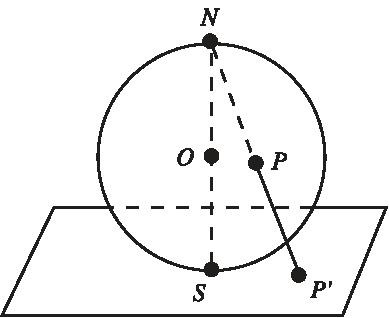
\includegraphics[width=90mm]{./algebraic_relationship_stereo.pdf}
\caption{}
\end{figure}

\begin{note}[Stereographic projection of $S^2$]

	The explicit map $p: S^2 \to \R^2 - \{ x \}$, $(x, y, z) \mapsto
	(\frac{2x}{1-z}, \frac{2y}{1-z})$, is derived from the algebraic relationship
	for each $P$ and $P'$, $P' - N = t(P - N)$ with fixed and real $t$, and the
	requirement that $P'$ lies on the $XY$ plane. See the image above.

	Work this out, good exercise.
\end{note}


\begin{note}[Interlude on quotient groups, relations, free groups]

Consider the free group on two generators, $Fr(a, b)$, and impose the
relation $a^3 = b^2$ (as in the torus knot $X_{3, 2}$.

This same relation can be induced by "factoring out" the normal subgroup
generated (conjugated by all elements in the group) by $a^3b^{-2}$. To see this, consider any word of the
generators, such as $a^ib^ja^3b^k$, and see for this word $a^ib^ja^3b^k (b^{-k}a^{-3}b^k) =
a^ib^jb^2b^k$. 

This idea is important in understanding abelianizations. The goal of the
abelianization of a group is to produce the smallest possible group where
elements commute, eg. $ab = ba$ for all $a, b \in G$. This is a relation, and
as before, we can induce the relation by the quotient of some group generated
by $aba^{-1}b^{-1}$. We just want to expand the generating subset to include
all possible pairs of elements (so that they all commute) but this generating
subset is the commutator subgroup, denoted $[G, G]$, given as $\{
aba^{-1}b^{-1} ~|~ a, b \in G\}$. $G \ [G, G]$ then gives a group with a new
set of relations that are the commutativity properties for all possible pairs
of elements.

(One thing that consistently tripped me up is the order of the elements in the
normal group $a^3b^{-2}$. The leftmost letter should intuitively be an inverse,
to "cancel out" and replace, eg. $a^3 (a^{-3}b^2) = b^2$. But $a^{-3} (a^3b^{-2}) a^3 = b^{-2}a^3$
is in our normal group as it is a conjugate. Similarly, generating our normal
group with $a^3b^{-2}$ (instead of $b^{-2}a^3$) produces an identical group.
This is a simple idea but one worth documenting for precision.
\end{note}

\begin{exercise}[1.2.10]
	Consider the arcs $\alpha$ and $\beta$ embedded in $D^2\times I$ as shown in
	Hatcher. A circle around the midpoint of the cylinder is nullhomotopic but
	show the same loop is not nullhomotopic in $D^2\times I - (\alpha \cap \beta)$
\end{exercise}

\begin{proof}
	Take one end of $\alpha$ and slide it towards the outside of the end of the
	cylinder, $D^2$, and then along the outside of the side of the cylinder,
	until it reaches the opposite cylinder end. This new cylinder is the
	complement of a straightened line and a loop $\beta$, and is homotopic to
	the original cylinder. In fact, these two spaces are homotopy equivalent, as
	composition of this initial sliding with the same sliding in reverse produces
	the original space, so they have isomorphic fundamental groups.

	Now repeat this procedure with $\beta$ and notice the
	final cylinder is the complement of two straightened lines. The fundamental
	group of this space is a free group on two generators. $\gamma$ belongs to
	the homotopy class of a loop of two generators in the final space. This new
	space is in isomorphic correspondence with the original cylinder, so
	$[\gamma] \neq 0$, and we have our result.
\end{proof}

\begin{note}Group descriptions of basic objects
	\begin{itemize}
		\item{$\pi_1(S^1) \cong \Z$}
		\item{$\pi_1(S^2) \cong 0$}
		\item{The fundamental group of a torus is $\pi_1(S^1 \times S^1) \cong \Z \star \Z$}
	\end{itemize}
\end{note}

We are now interested in how the fundamental group changes as we attach 2-cells
to a cell complex.

Let $X$ be some path connected space and $Y$ be the result of attaching a
collection of 2-cells $\{e^2_{\alpha}\}_{\alpha}$. The map $\varphi_{\alpha}:
S^1 \to X$, corresponding to each such $e^2_{\alpha}$, defines where it is
glued. The $\varphi_{\alpha}$ are loops that are not necessarily nullhomotopic
in $X$ but are certainly nullhomotopic when included in $Y$. Then
$\varphi_{\alpha}$ lie in the kernel of the isomorphism $\pi_1(X, x_0) \xhookrightarrow{} \pi_1(Y, y_0)$.

We will prove a stronger result, that the kernel of this isomorphism is exactly
the normal group generated by these loops (conjugated by the path $\gamma$ from
a basepoint on $\varphi$ to $x_0$). Let $N$ be the normal subgroup generated by
$\{ \gamma_{\alpha} \varphi_{\alpha} \bar{\gamma_{\alpha}}\}_{\alpha}$.

\begin{theorem}[van Kampen's applied to 2-dimensional cell complex]
	(a) the kernel of the isomorphism $\pi_1(X, x_0) \xhookrightarrow{} \pi_1(Y,
	y_0)$ is exactly $N$. So $\pi_1(X, x_0) / N \cong \pi_1(Y, y_0)$ 
	(b) Consider $Y$ obtained from $X$ with the same procedure, but $e^n$ for $n
	> 2$ used instead of $e^2$, then $N$ is trivial and $\pi_1(X, x_0) \cong
	\pi_1(Y, y_0)$.
	(c) For a path-connected cell complex $X$, the inclusion of its two-skeleton
	$X^2 \xhookrightarrow{} X$ induces an isomorphism $\pi_1(X^2) \cong
	\pi_1(X)$.
\end{theorem}

\begin{proof}

(a) We begin by constructing a space $Z$ from $Y$, by attaching strips $S_{\alpha}$
along each $\gamma$. (See Hatcher for a precise description of this
construction). What is more important is understanding why we do this, rather
than proceeding with van Kampen's on $Y$ itself.

Deconstruct $Z$ into $A = Z - \cup_{\alpha} y_{\alpha}$ (where each
$y_{\alpha}$ is a hole in the 2-cell $e^2_{\alpha}$) and $B = Z - X$. Notice
that $B$ is contractible, as a space of many 2-cells glued together, so
$\pi_1(B) = 0$. Verify quickly that $A$ and $B$ are open. $B$ is a set of
2-cells, which are open, attached to some closed strips, so $B$ is open. $A$ is
open as a two-skeleton with a finite number of holes.

When we setup the "van Kampen's homomorphism" in the standard
way, $\pi_1(A) \star \pi_1(B) \to \pi_1(Z)$, we obtain the isomorphism
$\pi_1(A) \ N \cong \pi_1(Z)$ where $N$ is generated by the image of $\pi_1(A \cap B) \to \pi_1(A)$. (This is a straightforward application of van Kampen's theorem).

See that for each $\gamma_{\alpha} \varphi_{\alpha} \bar{\gamma_{\alpha}}$, we
can obtain a corresponding $\delta_{\alpha} \in \pi_1(A \cap B)$ that travels along the
strip and around some concentric circle in the corresponding $e^2_{\alpha}$.
Indeed these loops are homotopic in $\pi_1(A \cap B)$ under a suitable
basepoint change isomorphism.

It remains to show that the image of $\pi_1(A \cap B) \to \pi_1(A)$ is
generated by these $\delta_{\alpha}$. We invoke van Kampen's again by
decomposing $A \cap B$ into $A_{\alpha} = A \cap B - \cap_{\beta \neq \alpha}
e^2_{\alpha}$. This time, each such $A_{\alpha} \cap A_{\beta}$ is
contractible, so $N$ is trivial. Each $A_{\alpha}$ deformation retracts to
$\varphi_{\alpha}$, so  $\pi_1(A_{\alpha}) \cong S^1$ or the group free on the
generator $\delta_{\alpha}$ (see this loop is homotopic to $\varphi_{\alpha}$).

(b) To see this result, we proceed with the same decomopositions as (a), but in
the second invocation of van Kampen's we notice each $A_{\alpha}$ is now some
n-cell with some hole, where $n > 2$, attached to many strips.
$\pi_1(A_{\alpha})$ is then trivial and so is $N$.

(c) When $n$ is finite, the result follows from straightforward induction using
(b). When $n$ is infinite, the author is frankly uninterested in understanding
the result at this time.
\end{proof}

\begin{theorem}
	If $g \neq h$, then $\pi_1(M_g)$ and $pi_1(M_h)$ are not isomorphic. Nor are the spaces homotopy equivalent.
\end{theorem}

\begin{proof}
	If $M_g \simeq M_h$, then their fundamental groups are isomorphic. These groups are the abelianizations of free groups in $2g$ and $2h$ generators respectively (this is immediate from the previous result). Because these groups are isomorphic, $g$ and $h$ must be the same.
\end{proof}

\begin{exercise}[1.2.14]
	Let $X$ be the cube, $I \times I \times I$, where each face is identified with
	its opposite face with a half twist. Show this quotient space is the
	cell complex with 2 0-cells, 4 1-cell, 3 2-cells and 1 0-cell. Using this
	structure show that $\pi_1(X)$ is the quanternion group of order 8.
\end{exercise}

\begin{proof}

	To first see the cell complex of $X$ is composed of the described n-cells, we
	draw a picture identifying the appropriate vertices and edges. The 2-skeleton
	of the cube collapses to a pair of vertices with four edges between them. The
	6 faces of the cube become 3 as we identify opposite pairs.

	Recall the fundamental group of a cell complex can be described by its
	2-skeleton as in $1.26$. Then $\pi_1(X) \cong \pi(X^1) / N$, where $X^1$
	is the 1-skeleton and $N$ is the normal group generated by loops of the
	attached 2-cells as in $1.26$. The single 3-cell has no effect on the
	fundamental group.

	Calculating $\pi_1(X^1)$ is a straightforward application of van Kampen's. We
	decompose $X^1$ into three open sets $A_1, A_2, A_3$, each obtained by tracing
	a different cycle through the two vertex graph $X$. If we assume $X$ inherits
	a metric topology from $\R^3$, these sets are open, and the intersection of
	any pair is a point. $\pi_1(A_1) \cong \pi_1(A_2) \cong \pi_1(A_3) \cong \Z$,
	so $\pi_1(X^1)$ is the group free on three generators.

	To construct $N$, it is sufficient to trace the attachment of 2-cells to the
	front, side and top face of the cube. If we do this, using the hand drawn
	image as a guide, we obtain $\{ abcd, adb^{-1}c^{-1}, b^{-1}dca^{-1} \}$ as
	the generators of $N$. $\pi_1(X)$ is then the free group on three generators
	with the relations induced by dividing by $N$:

	\[<ab, ac^{-1}, ad ~|~ abcd=adb^{-1}c^{-1}=b^{-1}dca^{-1}=1 >\]

	To see this group is isomorphic to $Q_8$, let $i=ab, j=ac^{-1}, k=ad$ and
	rewrite the above presentation:

	\[<i, j, k ~|~ ij^{-1}k=ki^{-1}j=i^{-1}kj^{-1}=1>\]

	We can rewrite the relations as $ij = k, i = jk, j = ki$ and then $k^2 = i^2
	= ijk$ (from the first and second relation). Obtaining $j^2 = ijk$ comes from
	$j = k(i) = k(jk)$, so $j^2 = (jk)jk = ijk$.

	\[<i, j, k ~|~ i^2=j^2=k^2=ijk> \cong Q_8 \cong pi_1(X) \]

\end{proof}

\begin{exercise}
	Show the fundamental group of the surface of infinite genus is free on
	infinite generators.
\end{exercise}

\begin{proof}
	First we show that for $M_1 - \{x, y\}$, the torus with two holes, $\pi_1(M_1
	- \{x, y\}) \cong \Z \star \Z$. To see this, consider the representation of a
	torus as a rectangle with opposite sides identified as in the figure. If we
	poke a hole in this shape, it deformation retracts to its 1-skeleton, which
	is the wedge sum $S^1 \vee S^1$. Poking an additional hole will not 
\end{proof}


\begin{figure}[ht!]
\centering
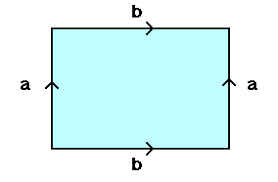
\includegraphics[width=90mm]{./torus.png}
\caption{}
\end{figure}

% HERE

% Problems

We will used the fact that a punctured n-sphere is homeomorphic to the 

\begin{proposition}[Proof of generalized stereographic projection]
There exists a homeomorphism between $S^n-1$ and
\end{proposition}

\begin{exercise}[1.2.4]
	Compute $\pi_1(\R^3 - X)$ where $X$ is the union of $n$ lines through the origin.
\end{exercise}

\begin{proof}
	Observe the complement deformation retracts to $S^2$ with $2n$ points removed (the poles of our $n$ lines). This object is homoemorphic to $\R^2$ with $2n-1$ points removed. (maybe construct the explicit stereographic projection). We can use van kampens to show the fundamental group of this space is the free group of $2n-1$ generators.
\end{proof}

\begin{exercise}[1.2.6]
	Supppose a space $Y$ is obtained from a path-connected space $X$ by attaching
	$n$-cells for a fixed $n \geq 3$. Then show the inclusion $X
	\xhookrightarrow{} Y$ induces an isomorphism on $\pi_1$. Use this result to
	then show	that the complement of a discrete subspace of $R^n$ is simply-connected if $n
	\geq 3$.
\end{exercise}

\begin{proof}

	We proceed using the structure of the proof of $1.26$. Let $A$ be $Y$ with a
	hole in each of the attached $n$-cells. Let $B$ be the union of the attached
	$n$-cells. See that $A$ and $B$ are both open and $Y = A \cup B$, so we
	invoke van Kampen's theorem: $\pi_1(Y) = \pi_1(A) \star \pi_1(B) / N$ where
	$N$ is defined in the usual way.

	As before, $A$ deformation retracts onto $X$, so $\pi_1(A) \cong \pi_1(X)$,
	and $B$ is contractible, so $\pi_1(B) = 0$. Then it remains to show that $N$
	generated by $\{ i_{AB}(\omega) i_{BA}(\omega)^{-1} | \omega \in \pi_1(A \cap
	B) \}$ is trivial (where the map $i_{AB}$ is defined as $i_{AB}: \pi_1(A \cap
	B) \to \pi_1(A)$). See that any loop $i_{AB}(\omega)$ is contractible,
	because despite introducing a hole, the loop can homotope around it within the
	interior of the $n$-cell (if $n \geq 3$). Any $i_{BA}(\omega)$ is trivially
	contractible, being included into an open subset of an $n$-cell with no
	holes. Then $\pi_1(Y) \cong \pi_1(X)$.

	% https://math.stackexchange.com/questions/1188062/why-is-the-complement-of-a-discrete-subspace-of-mathbbrn-n-ge-3-simpl

	To prove our last result, let $X$ be our space of interest (the complement of
	some discrete subspace of $R^n$), we can obtain a covering $\{ A_{\alpha} \}_{\alpha}$
	where each $A_{\alpha} = X - x_{\alpha}$ is the complement of each point in the discrete
	subspace. See each $A_{\alpha}$ is open. Then $\pi_1(Z) = \star \pi_1(A_{\alpha}) / N$.

\end{proof}

\begin{exercise}[1.2.7]
	Construct a cell complex for the two-sphere with north and south poles
	identified and use this to compute the fundamental group of this space.
\end{exercise}

\begin{proof}
	We first construct the cell complex. Begin with a 0-cell $x$ and attach a
	1-cell $e$ to $x$ to form a circle. Then take a 2-disk $\sigma$ and attach
	its boundary circle $\delta \sigma$ to $e$ in two pieces, $\delta_1 \sigma$
	traces one endpoint to the other and attaches to $e$, while $\delta_2 \sigma$
	completes the circle in the same orientation but attaches to $\bar{e}$.

	Then, by van Kampen's, our fundamental group is isomorphic to $< a ~|~ a a^{-1}
	>$, but this is just the free group on one generator, so $\pi_1(X) \cong \Z$.

\end{proof}

Seeing that the cell complex is the same as the sphere with north and south
poles identified was not immediately obvious.

\href{https://math.stackexchange.com/questions/1194611/cw-complex-structure-on-standard-sphere-identifying-the-south-pole-and-north-pol}{This
post} was helpful (notation was taken from Lee Mosher's solution), viewing our
space as the quotient map $f: D_2 \to X$ performing exactly two
identifications. 2-disks can take different forms equivalent up to
homeomorphism and their boundaries can simply be circles. Seeing that $S^2$ is
simply $D_2$ attached along $e$ and $\bar{e}$, where $e$ is an arc connecting
the poles, was crucial.


\begin{exercise}[1.2.8]

Consider a surface $M_g$ of genus $g$ that is split into two closed surfaces
$M_h$ and $M_k$ by a circle $C$. $M'_h$ and $M'_k$ are constructed by deleting an open disk
from each. Show that neither $M'_h$ or $M'_k$ retract to
their boundary circle, but both (and all of $M_g$) retract to a lateral $C'$.

% https://math.solverer.com/library/allen_hatcher/algebraic_topology/exercise_1-2-9
% https://math.stackexchange.com/questions/479371/how-to-construct-a-genus-2-surface-from-8-gon
% https://analysis-situs.math.cnrs.fr/Classification-des-surfaces-triangulees-par-reduction-a-une-forme-normale.html

\end{exercise}

More familiarity with the two torus (really genus g surfaces in general) and
practice with abelianization is needed to tackle this problem.

\begin{figure}[ht!]
\centering
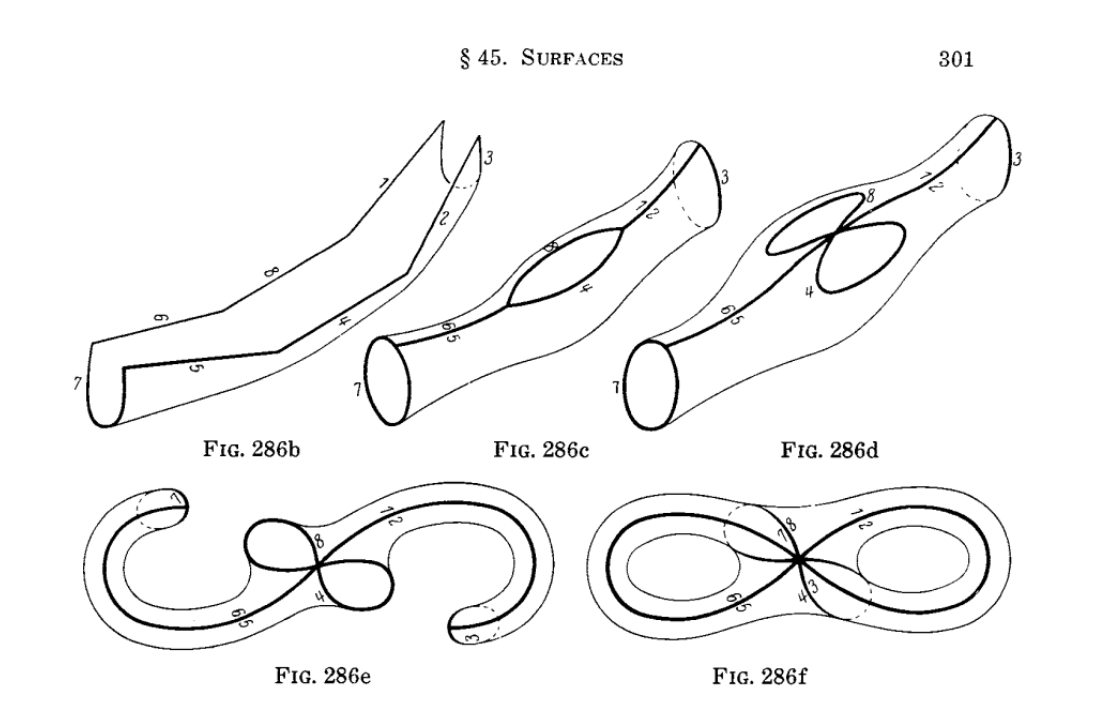
\includegraphics[width=90mm]{two-torus-hilbert.png}
\caption{The geometry of the two torus. Hilbert's \textit{Geometry and the Imagination} \label{overflow}}
\end{figure}

\begin{note}[Abelianization of $\pi_1(M_1)$]
	Consider $\pi_1(M_1) = < a, b ~|~ [a, b]$ as the familiar free group on two
	generators modulo the commutator (where $[a, b] = aba^{-1}b^{-1}$).

	The abelianization of $\pi_1(M_1)$ is then $\pi_1(M_1) \ [\pi_1(M_1), \pi_1(M_1)]$
\end{note}

\subsection{Covering Spaces}

Covering spaces let us (1) calculate fundamental groups of structures and (2)
think about algebraic properties using geometric intuition. (I do not really
understand how yet, so revisit this explanation after some exercise.)

\begin{definition}

	Given some space $X$, the space $\tilde{X}$, along with map $p: \tilde{X} \to
	X$, is a \textbf{covering space} if each $x \in X$ \textit{has some} open neighborhood
	$U$, where $p^{-1}(U)$ is a disjoint union of open sets and each one is
	mapped homeomorphically onto $U$ by $p$. These open sets are called
	\textbf{sheets}.
	
	$p^{-1}(U)$ is allowed to be empty, so $p$ need not be surjective.

\end{definition}

The helicoid (denoted $S$) is a good example that is easy to visualize. The helicoid can be
parameterized as: 

\[x = s \cos 2\pi t \]
\[y = s \sin 2\pi t \]
\[z = t \]

for $s \in (0, \infty), t \in \R$

\begin{figure}[ht!]
\centering
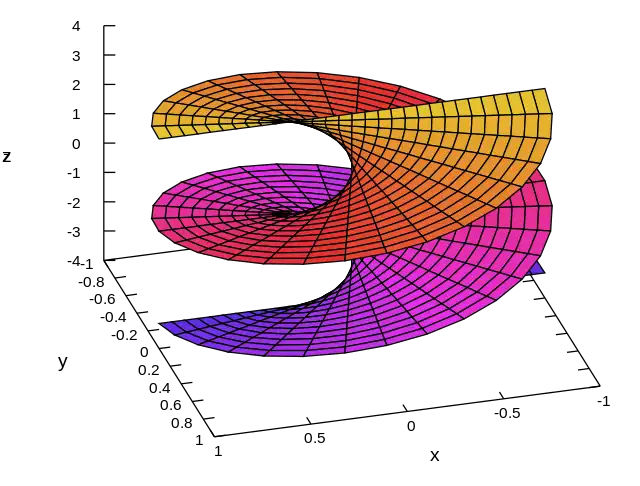
\includegraphics[width=90mm]{./helicoid.png}
\caption{}
\end{figure}

Then $p: S^1 \to \R \setminus \{0\}$ given by $(x, y, z) \mapsto (x, y)$ defines a
covering space of $\R - \{ 0 \}$.

I found this is best seen by looking at single line segments extending radially
from the origin. Consider $X = (0.5, 1.5) \times \{0\}$. $p^{-1}(X)$ is a
collection of disjoint segments. Our parameterization allows this segment of
the x axis to exist whenever we make one full rotation around the circle. There
are an infinite number of these segments and each maps to $X$ homeomorphically.

We can also look at the covering spaces of $S^1$. Let $p: S^1 \to S^1$ where
$p(z) = z \mapsto z^n$ with $z \in \Z$. Here $z \in S^1$ is the complex number
with $\abs{z} = 1$, so $S^1 = \{ z \in \C ~|~ \abs{z} = 1\}$.

Let $U = (0, \frac{\pi}{2})$ be some open segment of the circle, if $n=3$, what is
$p^{-1}(U)$?

Once place to see the utility of covering spaces is with oriented graphs.

\begin{figure}[ht!]
\centering
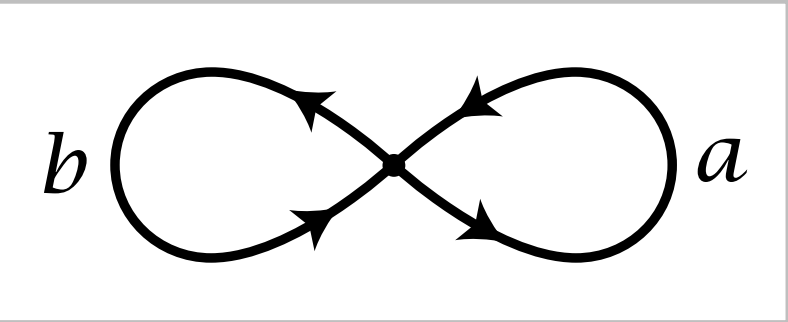
\includegraphics[width=90mm]{./2-oriented.png}
\caption{}
\end{figure}


Let $X$ (Fig. 3) be basepoint with two loops labeled $a$ and $b$. Now consider any
graph, $\tilde{X}$, where edge vertex has four edges. If we label, with $a$ or
$b$, and orient each edge we obtain a structure that looks like $X$ (respecting
orientation!) as we zoom into each vertex. We can call this an \textbf{2-oriented graph}.

If we construct a map $p: \tilde{X} \to X$, where the interior of each edge in 
$\tilde{X}$ maps homeomorphically to corresponding labeled edge in $X$
following the orientation of both edges, we satisfy the properties for a covering
space. It follows both that every oriented graph is a covering space of $X$ and
every covering space of $X$ can be 2-oriented (every vertex has 4 edges that
can be labeled so the local picture looks like $X$).

We are given a table of some of these $\tilde{X}$.

\begin{theorem}
	$\pi(X) \cong < a, b^2, bab^{-1} >$
\end{theorem}

\begin{proof}
Hatcher instructs us that we can use Van Kampen's.

% TODO - use the open sets from my notebook
\end{proof}

When we consider the fundamental group of the covering space as the "image
subgroup" of $\pi_1(X)$, $p_*(\pi_1(\tilde{X})) \leq \pi_1(X)$, we recover yet
another beautiful correspondence between algebra and geometry - there is a 
one to one correspondence between the subgroups $\pi_1(X)$ and covering spaces of $X$. 

A few more algebraic interpretations of covering spaces:

\begin{itemize}
	\item{If we change our basepoint in a covering space that is otherwise the
		same, $p_*(\pi_1(\tilde{X}, x_1))$ is a conjugacy subgroup of
		$p_*(\pi_1(\tilde{X}, x_0))$ in $\pi(X)$ where the conjugating element is the
	loop connecting the basepoints.}
\item{If a \textbf{symmetry} is an automorphism on a graph that preserves
		labels and orientations, then a graph can be "more" symmetric if it has
		more automorphisms and "the most" symmetric if every possible permutation
		of the graph vertexes have automorphisms with the desired properties. We
		will show that "the most symmetric" graphs are exactly those induced subgroups that
	are normal in $\pi_1(X)$.}
\end{itemize}

We now define three \textbf{lifting properties} of covering spaces and show
some applications. Given some covering space and a map into $X$, these
properties tell us when a lift of a homotopy exists, when a lift of a regular
map exists and when lifts are unique.

\begin{proposition}[Homotopy lifting property]
	Given a covering space $p: \tilde{X} \to X$, a homotopy $f_t: Y \to X$ and a
	lift of timepoint 0 of the homotopy $\tilde{f_0}: Y \to \tilde{X}$, there
	exists a \textit{unique} lift of the entire homotopy $\tilde{f_t}: Y \to X$.
\end{proposition}

When $Y$ is a point, this tells us that paths in $X$ induce unique paths in the
covering space.

When $Y$ is $I$, this tells us that homotopies in $X$ induce unique homotopies
in the covering space.

The key idea here is that these homotopies are unique. If we consider the lift
of a constant path, this implies that the lifted path is also constant 

\begin{note}
Check this. If $p\tilde{f} = f$ and $f$ is constant, if $\tilde{f}$ had anything
other than $\tilde{f}(0)$ in its image, what does that imply about the set of
allowed $\tilde{f}$s? If $\tilde{f}$ is itself constant, then $p\tilde{f} = f$
obvioulsy holds. 
\end{note}

We will use this to show $p_*$ is injective.

\begin{proposition}
	The induced homomorphism $p_*: \pi_1(\tilde{X}, \tilde{x_0}) \to \pi_1(X,
	x_0)$ is injective. The image subgroup $p_*(\pi_1(\tilde{X}, \tilde{x_0}))$
	consists of loops with baspoint $x_0$ that lift to loops in $\tilde{X}$ with
	basepoint $\tilde{x_0}$.
\end{proposition}

\begin{proof}
	To prove injectivity, consider two distinct homotopy classes, $[\tilde{f'_0}]$
	and $[\tilde{f''_0}]$, that have the same image under $p_*$, so
	$p_*([\tilde{f'_0}]) = p_*([\tilde{f''_0}])$. Indeed $p\tilde{f'_0} \simeq
	p\tilde{f''_0}$, given by some homotopy $f_t$, so our homotopy lifting
	property gives us a lifted homotopy $\tilde{f_t}$ where $\tilde{f'_0} \simeq
	\tilde{f''_0}$. Then $[\tilde{f'_0}] = [\tilde{f''_0}]$, so $p_*$ is
	injective.

	(This is a bit more explicit than Hatcher's proof using the kernel of $p_*$)

	A loop in $X$ with basepoint $x_0$ that lifts to a loop in $\tilde{X}$ with
	basepoint $\tilde{x_0}$ is by definition an element of $p_*(\pi_1(\tilde{X},
	\tilde{x_0}))$.

	The second statement is a bit bizarre, because should every element in the
	image subgroup, represented as $p_*\tilde{f}$, admit a straightforward lift
	$\tilde{f}$. I do not see where I have to invoke homotopy lifting, unless you
	consider some other representative of each homotopy class $g \simeq
	p\tilde{f}$, then $\tilde{g} \simeq \tilde{f}$, so the representative admits
	the desired lift.
\end{proof}

\begin{proposition}
	The number of sheets in a covering space $p$ is equal to the index of
	$p_*(\pi_1(\tilde{X}, \tilde{x_0}))$ in $\pi_1(X, x_0)$
\end{proposition}

\begin{proof}
	Let $g$ be a loop in $\pi_1(X, x_0)$. $\tilde{g}$ is its lift by the homotopy
	lifting property. Note that $\tilde{g}$ need not be a loop as $[g] \notin
	p_*(\pi_1(\tilde{X}, \tilde{x_0}))$! (Consider the lift
	of a single wrap around the circle in $p: \R \to S^1$.)

	Each representative of our coset $H = p_*(\pi_1(\tilde{X}, \tilde{x}))$ can
	be denoted $H[g] = h\cdot g$, which has a lift $\tilde{h}\cdot\tilde{g}$.
	$\tilde{h}$ is a loop at $\tilde{x}$ by the prior theorem, so notice that
	$\tilde{h}\cdot\tilde{g}$ is a path that starts at $\tilde{x_0}$ and ends at
	$\tilde{g}(1)$.

	We claim that these cosets are one to one with the preimage of
	basepoints $p^{-1}(x_0)$. Consider the function $\phi = [H]g \mapsto
	\tilde{g}(1)$. It is well-defined as for $hg, h'g \in [H]g$, $\phi(hg) =
	\phi(h'g) = g(1)$.

	$\tilde{X}$ is path-connected so the path $\tilde{g}$ can be extended to any
	point in $p^{-1}(x_0)$, so $\phi$ is surjective. To see $\phi$ is injective,
	if $\phi([H]g) = \phi([H]g')$, then $g(1) = g'(1)$, so $g\cdot\bar{g'}$ is a
	loop with basepoint $x_0$ that lifts to a loop with basepoint $\tilde{x_0}$.
	Then $g\cdot\bar{g'} \in H$ and $[H]g = [H]g'$.
\end{proof}

We have two more properties. One will show when a lift exists and another will
show when lifts are unique.

\begin{proposition}[Lifting criterion]
	Given a covering space $p: \tilde{X} \to X$ and some map $f: Y \to X$, there
	exists a lift of this map, denoted $\tilde{f}: Y \to \tilde{X}$, iff $f_*(\pi_1(Y, y_0)) \subseteq
	p_*(\pi_1(\tilde{X}, \tilde{x_0}))$.
\end{proposition}

\begin{proof}
	The necessary condition is straightforward. The existence of a lift implies
	that $f = p\tilde{f}$, then $f_* = p_*\tilde{f_*}$. Then for any loop $\gamma: I
	\to Y$ in $\pi_1(Y, y_0)$, $p_*^{-1}f_*(\gamma) = \tilde{f_*}(\gamma)$.
	Certainly $f_*(\pi_1(Y, y_0)) \subseteq p_*(\pi_1(\tilde{X}, \tilde{x_0}))$.

	The sufficient condition is less straighforward. We proceed by constucting
	our lift $\tilde{f}$ explicitly. Let $\tilde{f} = y \mapsto \tilde{f\gamma}(1)$,
	where $\gamma$ is any path from $y_0$ to $y$. We will show that this function
	is well-defined - that it does not matter what path we draw to $y$. 

	Consider another path $\gamma'$. We build a loop $\gamma \cdot
	\bar{\gamma'}$.  Consider $f(\gamma \bar{\gamma'})$, which is also a loop. By
	assumption, this is some element of $p_*(\pi_1(\tilde{X}, \tilde{x_0}))$,
	call it $[ x ]$, so $f(\gamma \bar{\gamma'})$ homotopes to $x$. Because $x$
	lifts to a loop with basepoint $\tilde{x_0}$, by the homotopy lifting
	property, $f(\gamma \bar{\gamma'})$ itself lifts to a loop with basepoint
	$\tilde{x_0}$. So for $\tilde{f}(\gamma \bar{\gamma'})$,
	$\tilde{f}(\gamma)(1) = \tilde{f}(\bar{\gamma'})(0)$ and
	$\tilde{f}(\gamma)(1) = \tilde{f}(\gamma')(1)$ as desired.

	We must also check for continuity. Consider some open $U$ about $f(y)$ that
	is mapped homeomorphically to its lift $\tilde{U}$ about $\tilde{f}(y)$ by
	$p: \tilde{U} \to U$. By continuity of $f$, there exists some $N$ about $y$
	where $f(N) \subset U$. We will see that $\restr{\tilde{f}}{N} = p^{-1}f$.
	$N$ is path connected, so let $\eta$ to be the path from $y$ to any $y' \in
	N$ ($\gamma$ is still the path from $y_0$ to $y$), then $\tilde{f}(N) =
	p^{-1}f(N)$ (Varying $\eta$, $\tilde{f\cdot\eta}(1)$ are exactly the points
	mapped onto $\tilde{N}$ by $p^{-1}$. This is true for arbitrary $N$.
\end{proof}

\begin{proposition}[Unique lifting property]
	Given a covering space $p: \tilde{X} \to X$ and some map $f: Y \to X$, if
	$\tilde{f_1}$ and $\tilde{f_2}$ agree on one point of $Y$ and $Y$ is
	connected, they agree on all of $Y$.
\end{proposition}

\begin{proof}
	For a point $y \in Y$ let $U$ be an evenly-covered neighborhood of $f(y)$
	(recall this means that $p^{-1}(U)$ is a set of open sets in $\tilde{X}$ each
	mapping homeomorphically to $U$). Let $\tilde{U_1}$ and $\tilde{U_2}$ be the
	open sets that $\tilde{f_1}(y)$ and $\tilde{f_2}(y)$ reside in respectively.

	If $\tilde{f_1}(y) \neq \tilde{f_2}(y)$, then $\tilde{U_1} \neq \tilde{U_2}$
	so these sheets are disjoint.

	Consider an open $N$ about $y$ that maps into $\tilde{U_1}$ and $\tilde{U_2}$
	by each lift. Such an $N$ exists because of continuity. If $\tilde{f_1}(y)
	= \tilde{f_2}(y)$, then $N$ must map into the same $\tilde{U}$. Because
	$p\tilde{f_1} = p\tilde{f_2}$ and $p$ is injective over over $\tilde{U}$ (it
	is homeomorphic with $U$), these lifts agree over $N$.
\end{proof}

\begin{definition}[semilocal simple connectedness]
	For each point $x \in X$, there exists $U$, where $\pi_1(U)
	\xhookrightarrow{}{\pi_1(X)}$ induced by the inclusion map is trivial.
\end{definition}

Notice that this does not mean that $U$ itself is simply connected, rather that
loops within $U$ can homotope throughout the whole space to $X$.

For a fixed, path-connected $X$, we are now interested in classifying the
various covering spaces. The main result is a correspondence between subgroups
of $\pi_1(X, x_0)$ and covering spaces $p: tilde{X} \to X$, where
$p_*(\pi_1(\tilde{X}))$ is equivalent to each subgroup. We are first interested
in constructing the trivial subgroup for arbitrary $X$. Since we have shown
that $p_*$ is always injective, it is sufficient to construct a simply-connected covering space $\tilde{X}$.

\begin{example}[Constructing the universal cover]
	What follows is a rather abstract procedure for building this
	simply-connected space, called the \textbf{universal cover}, for a
	path-connected, locally path-connected and semilocally simply-connected space
	$X$.

	First, recall that there is a single homotopy class of paths for fixed
	endpoints in a simply connected space. If $\tilde{X}$ is simply-connected and 
	we fix some basepoint $\tilde{x_0}$, then for each point $x \in \tilde{X}$, a path
	$\gamma$ from $x_0$ to $X$ uniquely defines $[\gamma]$. The set of $[\gamma]$ is
	bijective with $\tilde{X}$. By the homotopy lifting property, homotopy
	classes of paths starting at $x_0$ in $X$ lift uniquely to homotopy classes of paths
	in $\tilde{X}$ starting at $\tilde{x_0}$. This gives a way to build
	$\tilde{X}$ from just $X$. (But this does not mean that $\gamma(1)$ uniquely
	defines each point.)

	\[\tilde{X} = \{ [\gamma] ~|~ \gamma \text{is a path in } X \text{ starting at } x_0\]

	Let $p = [\gamma] \mapsto \gamma(1)$ be our covering map. $p$ is surjective
	because $X$ is path connected. We can have many distinct $[\gamma]$, all with
	the same endpoint, so $p$ is certainly not injective (but most covering
	spaces are not so this is fine.

	Now we make use of the semilocally simply-connected property. Let
	$\mathcal{U}$ be the collection of $U$ where $\pi_1(U) \to \pi_1(X)$ is
	trivial. Notice that $\mathcal{U}$ is a basis for the topology of $X$. Every
	$x \in X$ has some $U$ about it that satisfies this property and for each
	each pair of $U_1, U_2 \in \mathcal{U}$ and $x \in U_1 \cap U_2$, there
	exists $U_3 \in \mathcal{U}$ where $x \in U_3 \subseteq U_1 \cap U_2$
	($\pi_1(U_3) \to \pi_1(U_1 \cap U_2) \to \pi_1(U_1) \to \pi(X)$ is a chain of
	trivial homomorphisms induced by inclusions)

	We need to now define a topology on $\tilde{X}$. Then show that $p$ has the
	properties of a covering map (continuous + disjoint sheets). We define:

	\[U_{[\gamma]} = \{ [\gamma \cdot \eta ~|~ \eta \text{ is a path within } U \text{ where } \eta(0) = \gamma(1) \}\]

	See that restricting $p$ to each $U_{\gamma}$ now gives us a bijection.
	Surjectivity, as before, comes from $U$ being path-connected. But now, if 
	$[\gamma'] \neq [\gamma'']$, because $\pi_1(U)$ is trivial under inclusion,
	these paths must have different endpoints. So $p$ is injective.

	To prove one of the properties of a basis, we show in general that $U_{[\gamma]} = U_{[\gamma']}$ if $[\gamma'] \in
	U_{[\gamma]}$ (Certainly $U_{[\gamma']} \subseteq U_{[gamma]}$ as $[\gamma
	\cdot \eta' \cdot \eta''] = [\gamma \cdot \eta]$. Similarly $U_{[\gamma]}
	\subseteq U_{[gamma']}$ as $[\gamma \eta ] = [\gamma \cdot \eta \cdot
	\bar{\eta} \cdot \eta']$).

	Then, varying over $U \in \mathcal{U}$ and $[\gamma]$ that induce distinct
	$U_{[\gamma]}$ for fixed $U$, $\{ U_{[\gamma]} \}$ defines our topology on
	$\tilde{X}$. Every $[\gamma]$ has such a set. For $[\gamma''] \in
	U_{[\gamma]} \cap V_{[\gamma']}$, let $W \subseteq U \cap V$ contain
	$\gamma''(1)$. Then $[\gamma''] \in W_{[\gamma'']} \subseteq U_{[\gamma'']}
	\cap V_{[\gamma'']} = U_{[\gamma]} \cap V_{[\gamma']}$.

	We now show that $p: U_{[\gamma]} \to U$ is also a homeomorphism. In other
	words, open $V \subseteq U$ are one-to-one with $V_{[\gamma]}$. Indeed,
	$p(V_{[\gamma]}) = V$. Similarly, $p^{-1}(V) \cap U_{[\gamma]} =
	V_{[\gamma]}$.

	This is what we need to prove that $p$ is a covering space. $p$ is 
	continuous, as we have showed $p$ to be a homeomorphism when restricted to each element of the
	basis for $\tilde{X}$. To see $p^{-1}(U)$ is a set of disjoint sheets, see
	that $U_{[\gamma]}$ partitions this set as we vary $\gamma$. Indeed if
	$[\gamma''] \in U_{[\gamma]} \cap U_{[\gamma']}$, then $U_{[\gamma]} =
	U_{[\gamma'']} = U_{[\gamma']}$. (Stop and think about what disjoint sheets
	imply about $\gamma$ for fixed $U$).

	Finally we show that $\tilde{X}$ is simply-connected. See first that for some
	path $\gamma$ in $X$, a lift of this path in $\tilde{X}$ can be described by
	the function $t \mapsto [\gamma_t]$ where $\gamma_t$ is $\gamma$ during $[0,
	t]$ but constant during $[t, 1]$. Now we show that $p_*(\pi_1(\tilde{X}),
	\tilde{x}_0)$ is trivial, and because $p_*$ is injective, this gives us our
	result. Consider an element $g \in p_*(\pi_1(\tilde{X})$, a loop at $x_0$
	that lifts to a loop in $\tilde{X}$. This lift goes from $[x_0]$ to $[g_1]$,
	using the definition at the beginning of the paragraph,
	but $[g_1] = [x_0]$ because it is a loop. This is true for arbitrary $[g_1] =
	[g]$.
\end{example}

\begin{example}
	Let $X_{m,n}$ be the quotient space of a cylinder $S^1 \times I$ with the
identifications $(z, 0) \simeq (e^{\frac{2\pi i}{m}}z, 0)$ and $(z, 1) \simeq
(e^{\frac{2\pi i}{n}}z, 1)$. Note $z$ is a complex coordinate and the
transformation is a $\frac{1}{n}$ twist.

	$A$ and $B$ are subspaces of $X$ and the quotients of $S^1 \times [0, \frac{1}{2}]$ and $S^1
	\times [\frac{1}{2}, 1]$ respectively. One end of each half cylinder is just
	the circle ($A \cap B = S^1$), but they "twist" to the identification.

	See that if $m = n = 2$, then $A$ and $B$ are the mobius band.

	% TODO, see that both of them combined are the klein bottle
	% - Revisit the construction of non orientable surfaces by gluing disks onto
	% circles
	% - The boundary of a mobius strip is homeomorphic to circle
	% - In fact the boundary of each of 1.29 is a circle
	% - Walk through connection between projective plane and mobius strip
  %   Helpful! https://www.youtube.com/watch?v=B6vEdfk7SWU
	% ( https://www.groupoids.org.uk/outofline/motion.html#motion )
\end{example}

The procedure used to build the universal cover can be used to complete the
rest of the subgroups.

\begin{theorem}
	For each $H \leq \pi_1(X, x_0)$, there exists a covering space $p_*: X_H \to
	X$ where $p_*(\pi_1(X_H, \tilde{x_0})) = H$ for a suitably chosen basepoint
	$\tilde{x_0}$. 
\end{theorem}

\begin{proof}

	Our strategy is to construct a quotient space out of our universal cover.

	For $[\gamma], [\gamma'] \in \tilde{X}$ (remember that these are in fact
	points), let $\gamma \sim \gamma'$ if $\tilde{\gamma}(1) =
	\tilde{\gamma'}(1)$ and $[\gamma \bar{\gamma'}] \in H$.

	First we define an equivalence class as $[\gamma] \sim [\gamma']$ if and only
	if $[\gamma \cdot \bar{\gamma'}] \in H$. We omit the proof of reflexivity,
	transitivity and symmetry as it is easy to see.

	We then take our universal cover $tilde{X}$ and identify points that belong
	in this equivalence class. Observe that this 

	For $[\gamma] = [c \cdot \gamma] \in H$ (where $[c]$ is the equivalence class
	of the identity), then $[c] \sim [\gamma]$.

\end{proof}

We are interested in constructing isomorphisms between different covering
spaces so we can use these to classify them. We define an isomorphism between
covering spaces $p_1: \tilde{X_1} \to X$ and $p_2: \tilde{X_2} \to X$ as a
homeomorphism $f: \tilde{X_1} \to \tilde{X_2}$ where $p_1 = p_2 \cdot f$.
Notice that this homeomorphism preserves the covering space structure, eg.
fibers $p_1^{-1}(x_0)$ are mapped to fibers $p_2^{-1}(x_0)$.

When do these isomorphisms exist?

\begin{exercise}
	If $p_1: \tilde{X_1} \to X$ and $p_2: \tilde{X_2} \to X$ are two covering
	spaces for the path-connected and locally path-connected $X$ with basepoint
	$x_0$. Then we can construct an isomorphism $f: \tilde{X_1} \to \tilde{X_2}$, mapping
	$\tilde{x_1} \in p_1^{-1}(x_0)$ to $\tilde{x_2} \in p_2^{-1}(x_0)$, iff
	$p_1*(\pi_1(\tilde{X_1}, \tilde{x_1})) = p_2*(\pi_1(\tilde{X_2}, \tilde{x_2}))$.
\end{exercise}

\begin{proof}
	To see the forward direction, consider the existence of $f$:
	\[
	\begin{tikzcd}
	\tilde{X_1} \arrow[r, "p_1"] \arrow[d, "f" description] & X \\
	\tilde{X_2} \arrow[ru, "p_2"']                          &  
	\end{tikzcd}
	\]

	Because $p_1f = p_2$, $p_1*(\pi_1(\tilde{X_1}, \tilde{x_1})) \subseteq
	p_2*(\pi_1(\tilde{X_2}, \tilde{x_2}))$. Using a symmetric argument with
	$p_2f^{-1} = p_1$, see $p_1*(\pi_1(\tilde{X_1}, \tilde{x_1})) = p_2*(\pi_1(\tilde{X_2},
	\tilde{x_2}))$.

	To see the reverse, notice that $p_1*(\pi_1(\tilde{X_1}, \tilde{x_1})) = p_2*(\pi_1(\tilde{X_2}, \tilde{x_2}))$ gives us lifts of both $p_1$ and $p_2$
	by the lifting criterion.

		\[
	\begin{tikzcd}
	\tilde{X_1} \arrow[r, "p_1"] \arrow[d, "\tilde{p_1}"', bend right]   & X \\
	\tilde{X_2} \arrow[ru, "p_2"'] \arrow[u, "\tilde{p_2}"', bend right] &  
	\end{tikzcd}
	\]

	Because $p_1 = p_2 \tilde{p_1}$ and $p_2 = p_1 \tilde{p_2}$, substitution gives
	us $p_2 = p_2 \tilde{p_1}\tilde{p_2}$ so $\tilde{p_1}\tilde{p_2} = 1$. A
	symmetric substituion gives us $\tilde{p_2}\tilde{p_1} = 1$, so the lifts are
	inverse isomorphisms and we have our result.

\end{proof}

We conclude with the final classification theorem.

\begin{theorem}
	There is a bijection associating the basepoint-preserving isomorphism classes
	of path-connected covering spaces $p: (\tilde{X}, \tilde{x_0}) \to (X, x_0)$
	with the set of subgroups of $\pi_1(X, x_0)$ obtained by associating the
	subgroup $p_*(\pi_1(\tilde{X}, \tilde{x_0}))$ with the covering space
	$(\tilde{X}, \tilde{x_0})$. 

	If we ignore basepoints, we obtain an association with conjugacy classes of
	subgroups of $\pi_1(X, x_0)$ and (basepoint-changing) isomorphism classes $p:
	\tilde{X} \to X$.
\end{theorem}


Another way to classify \textbf{disconnected} covering spaces of a space $X$
is by permutations of the fiber $p^{-1}(x_0)$ for a suitable basepoint. We
motivate this with a few specific examples before deriving a general construction
similar to the one used to build the universal cover.

\begin{figure}[ht!]
\centering
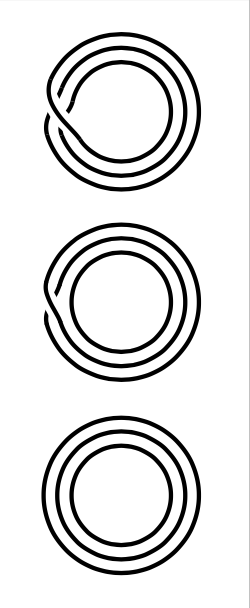
\includegraphics[width=20mm]{3-component-covering-spaces-of-s1.png}
\caption{The three different 3 component covering spaces of the circle}
\end{figure}

\begin{note}
	For some space $X$ and baspoint $x_0$, consider the 3 component covering
	spaces of $S^1$, denoted $\tilde{X_1}, \tilde{X_2}, \tilde{X_3}$, where the
	subscript indicates the number of components. Let $p^{-1}(x_0)$ be the fiber
	of $p$ and notice it is just three points for all $\tilde{X_n}$. For each
	covering space, the lift of the generator of $\pi_1(S^1)$ induces a
	permutation of the fiber. There are three starting points in $p^{-1}(x_0)$ it
	may start and the end of the lift is another point in $p^{-1}(x_0)$,
	potentially the same point.

	Notice the types of permutations $p$ induces is different for each
	$\tilde{X_n}$. $\tilde{X_3}$ induces cyclical permutations on all three points.
	$\tilde{X_2}$ induces cyclical permutations on two points with the third
	fixed. $\tilde{X_1}$ induces only the identity permutation.
\end{note}

In fact, disconnected covering spaces of $S^1$ are efficient graphical
representations of the different permutations of the fiber $p^{-1}(x)$.
This is also true for $S^1 \vee S^1$ (and perhaps true for all such spaces
where the fundamental group is free on some generators). 

This is no longer true if the covering space must be connected. For example,
with the 3 component covering space of $S^1$, the generator must lift to some
permutation of all basepoints otherwise the space is disconnected.

We can generalize this idea that "covering spaces are just permutations" with
the following idea. Consider $\gamma \in \pi_1(X, x_0)$, and notice each
$\tilde{gamma}$ (there can be many) starts at some $p^{-1}(\gamma(0))$ and this
choice of starting point defines where it ends in $p^{-1}(\gamma(1))$. We can
define a bijective function $L_{\gamma}: p^{-1}(\gamma(0)) \to p^{-1}(\gamma(1))$.

In fact, each $\tilde{X}$ defines a unique set of $L_{\gamma}$ that correspond
to each $[\gamma] \in \pi_1(X)$. All we have done is formalized the idea that
we can construct many unique covering spaces from the same space using
different ways of connecting the points in the fiber.

One important modification is to make composition of $L_{\gamma}$ respect the
direction of path composition. $\gamma \cdot \eta$ goes left to right, but
$L_{\gamma \eta} = L_{\gamma}\cdot L_{\eta}$ is the opposite direction. If we
define $L_{\gamma}$ as $p^{-1}{\gamma(1)} \to p^{-1}{\gamma(0)}$ instead,
composition of functions respects composition of paths.

The n-sheeted covering spaces of $X$ are then described by the homomorphisms
$\pi_1(X, x_0) \to Sym(n)$ defined as $\gamma \mapsto L_{\gamma}$. Here
$Sym(n)$ is the permutation group of $n$ items.

--

For a given covering space $\tilde{X} \to X$, the set of isomorphisms,
$\tilde{X} \to \tilde{X}$, actually have a name and themselves form a group
$G(\tilde{X})$. We call these \textbf{deck transformations}.

Note that, assuming $\tilde{X}$ is path connected, each deck transformation is
uniquely determined by where it maps a single point, if $\tilde{X}$ is path
connected, so we will often work with basepoints without losing information.
(To see this, consider the isomorphism as a lift and use the unique lifting
criterion to show it is uniquely determined by where it maps one point).

We call a covering space \textbf{normal} if for each point $x \in X$, there
exists a deck transformation between each pair of lifted points $\tilde{x},
\tilde{x'} \in \tilde{X}$. We will now show a correspondence between this
geometric concept and the familiar algebraic property.

\begin{definition}
	Let $p: \tilde{X} \to X$ be a covering space. Let $H = p_*(\pi_1(\tilde{X},
	\tilde{x_0}))$ be a subgroup of $\pi_1(X, x_0)$.
	\begin{itemize}
		\item{$\tilde{X}$ is a normal covering space iff $H \trianglelefteq \pi_1(X, x_0)$}
	\end{itemize}
\end{definition}

\begin{proof}
	We have already shown in the classification theorem that basepoint changes in
	a covering space correspond to a conjugate subgroup of $H$. In particular,
	for some $[\gamma] \in \pi_1(X, x_0)$, that lifts to the path $\tilde{\gamma}$ in
	$\tilde{X}$ traveling from $\tilde{x_0}$ to $\tilde{x_1}$,
	$[\gamma]H[\bar{\gamma]} = p_*(\pi_1(\tilde{X}, \tilde{x_1}))$. Then
	$[\gamma]$ is in the normalizer of $\pi_1(X)$, $N(G)$, iff 
	$p_*(\pi_1(\tilde{X}, \tilde{x_0}) = p_*(\pi_1(\tilde{X}, \tilde{x_1})$.
	We know from the unique lifting criterion that this relation induces a deck
	transformation mapping $\tilde{x_0}$ to $\tilde{x_1}$. Then if $N(G) =
	\pi_1(X)$ or $H \trianglelefteq \pi_1(X)$.

	To see the second claim, it is useful to start with the map $\varphi: N(G) \to
	G(\tilde{X})$, mapping each $[\gamma]$ to its deck transformation induced by the
	lifted loop. This is a surjective map because, as we just showed, all such deck
	transformations are exactly the members of $N(G)$. It is also a homomorphism.

	Let $\gamma$ lift to $\tilde{\gamma}$ from $\tilde{x_0}$ to $\tilde{x_1}$
	corresponding to deck transformation $\tau$ and
	consider another $\gamma'$ that lifts to $\tilde{\gamma'}$ from $\tilde{x_0}$
	to $\tilde{x_1'}$ corresponding to deck transformation $\tau'$.
	$\varphi([\gamma][\gamma'])$ 
	$\varphi([\gamma])\varphi([\gamma']) = \tau\tau'$ which agrees on $x_0$.

	Consider $\ker \varphi$, and notice these are exactly the loops that lift to
	loops, so $\ker \varphi = H$. Then $N(G) / H \simeq G$.
\end{proof}

Notice that deck transformations, as group of homeomorphisms on a topological
space, are a special case of the familiar algebraic notion of group actions.
There is a homomorphism $p: G \to Homeo(Y)$, $g \mapsto Y \to Y$, and assuming
$Y$ is path-connected and therefore deck transformations are unique, $p$ is
injective and $G$ is a subgroup of $Homeo(Y)$.

There is an important property that deck tranformations intuitively satisfy.
They map the sheets of the covering space to completely different sheets.

% TODO describe

It turns out that 

\begin{definition}
	For a group $G$ acting on $Y$ and satisfying $(*)$.
	\begin{itemize}
		\item{$p: Y \to Y\ G$ is a normal covering space}
		\item{$G$ is exactly the deck transformation group of $p$ if $Y$ is path-connected}
	  \item{If $Y$ is also locally path-connected, then $\pi_1(Y\ G)/p_*(\pi_1(Y)) \cong G$}
	\end{itemize}
\end{definition}

\begin{proof}
% TODO describe
\end{proof}

\begin{exercise}
	Let $Y$ be a subset of $\R^2$ that consists of a portion of the function
	$\sin(\frac{1}{x})$, the segment $L = [-1, 1]$ in the y-axis and an arc
	connecting these pieces. Let $f: Y \to S^1$ be the quotient map collapsing
	the segment to a single point. Show that $f$ does not lift to the covering
	space $\R \to S^1$ despite $\pi_1(Y) = 0$. (Then $f_*(\pi_1(Y)) \subseteq
	p_*(\pi_1(\tilde{X})$ would be trivial and we should have our lift be
	Proposition 1.36). Indeed local path connectedness is a necessary property
	for the lifting criterion.
\end{exercise}

\begin{proof}
	The problematic component is $L$. Assume we have a lift $\tilde{f}$. We first
	observe that $\tilde{f}(L)$ must be a single point. By definition of the
	quotient map $f$ assume $f(L) = \{1\}$ ($1 = e^{0i}$ or the top point of
	$S^1$ and the choice of point does not matter) and see $p^{-1}(\{1\})$ is a
	disjoint set of points in $\R$.  Because $L$ is connected, $\tilde{f}(L)$
	must also be a single point.

	Now see that $\tilde{f}(Y / L)$ must lie in a single component of $p^{-1}f(Y
	/ L)$ because $Y / L$ is connected. $f$ is surjective and $f(Y / L)$ is $S^1
	- \{0\}$, so $\tilde{f} = p^{-1}f(Y/L) = (0, 2\pi)$. However, because $Y$ is
	compact, $\tilde{f}(Y)$ must also be compact and $[0, 2\pi] \subseteq
	\tilde{f}(Y)$ (certainly $(0, 2\pi) \neq \tilde{f}(Y)$. (It is important to
	see that this would not be true if $L$ was already collapsed to a point in
	$Y$. See the note below). Then $\{ 0, 2\pi \} \in \tilde{f}(L)$, a
	contradiction.
\end{proof}

\begin{note}
	While $[-1, 1] \cup \{ (x, \frac{1}{x}) | x \in (0, 1] \}$, the topologist's
	sin curve, is compact, $[-1, 1] \cup \{ (x, \frac{1}{x}) | x \in (0, 1] \}$,
	the topologist's sin curve with the leftmost edge collapsed to a point, is
	not compact.
\end{note}

We will use some results about homotopy inverses from Chapter 0.

\begin{exercise}
	Show that for $f: X \to Y$ and $g, h: Y \to X$, $f$ is a homotopy equivalence if $fg
	\simeq 1_Y$ and $hf \simeq 1_X$.

	More generally, if $fg$ and $hf$ are homotopy equivalences, $f$ is also a
	homotopy equivalence.
\end{exercise}

\begin{proof}
	The map $hfg$ satisfies the requried homotopy equivalence properties - $f \cdot hfg
	\simeq 1_X$ and  $hfg \cdot f \simeq 1_Y$. To see this, $fhfg \simeq f1_Xg
	\simeq fg \simeq 1_Y$. A symmetric argument is used for the second
	equivalence.

	There is also a more straightforward proof for the first part. $g \simeq gfh \simeq h$ so certainly
	$gf \simeq 1_X$.

	To see the second result, we can use just $fg$. $fgi \simeq 1_Y$, so $gi$ is
	a candidate for the inverse. To see $gif \simeq 1_X$, observe $ifg \simeq
	1_Y$ by definition, so by left composition of $g$, $gifg \simeq g$ so $gif
	\simeq 1_X$.
\end{proof}

Notice that we can swap out functions in compositions and preserve
equality up to homotopy.

\begin{exercise}
	Let $\tilde{X}$ and $\tilde{Y}$ be simply-connected covering spaces of the
	path-connected, locally path-connected spaces $X$ and $Y$. Show that if
	$X \simeq Y$ then $\tilde{X} \simeq \tilde{Y}$.
\end{exercise}

\begin{proof}

	Define $p_X$ and $p_Y$ using the commutative diagram below:

	\[
\begin{tikzcd}
\tilde{X} \arrow[dd, "p_X"']                                      &  & \tilde{Y} \arrow[dd, "p_Y"]                                         \\
                                                                  &  &                                                                     \\
X \arrow[rr, "f", bend left] \arrow[rruu, "\tilde{f}", bend left] &  & Y \arrow[ll, "g", bend left] \arrow[lluu, "\tilde{g}"', bend right]
\end{tikzcd}
\]

	First see $f$ and $g$ have lifts as the necessary criteria from the existence
	theorem are satisfied. $X$ and $Y$ are both path-connected and
	locally path-connected, and certainly $f_*(\pi_1(X)) \subseteq
	p_{Y*}(\pi_1(\tilde{Y}))$ as $\tilde{X}$ is simply connected (a symmetric
	claim holds for $Y$).

	Observe $gfp_X \simeq 1_Xp_X \simeq p_X$. Using the existence of lifts for $g$ and
	$f$, we can expand the maps to arrive at $p_X\tilde{g}p_Y\tilde{f}p_X$. We
	can can then regroup our maps to arrive at the desired relation
	$p_X\tilde{g}p_Y\tilde{f}p_x \simeq p_X(1_{\tilde{X}})$.  Indeed,
	$\tilde{g}p_Y\tilde{f}p_x \simeq 1_{\tilde{X}}$. Repeating this procedure for
	$fgp_Y \simeq p_Y$ we recover the relation $\tilde{f}p_X\tilde{g}p_Y \simeq
	1_{\tilde{Y}}$. So $p_X\tilde{f}: \tilde{X} \to \tilde{Y}$ and $p_Y\tilde{g}:
	\tilde{Y} \to \tilde{X}$ are homotopy inverses.
\end{proof}


\begin{exercise}
	Find all the 2-sheeted and 3-sheeted connected covering spaces of $S^1 \vee
	S^1$, up to isomorphism of the covering spaces without basepoints.
\end{exercise}

\begin{proof}
	For the 2-sheeted covering spaces, we will try to use the different
	permutations of the fiber $p^{-1}(x)$ to identify possibilities. Let $Sym(2)$
	be the permutation group of order $2$ that contains just the identity map and
	transposition. Because $\pi_1(S^1 \vee S^1) \cong a \star b$, we can
	construct homomorphisms into $Sym(2)$ be mapping each of the generators, $a$
	and $b$ onto 
	
	% TODO
\end{proof}

\begin{exercise}
	Construct finite graphs $X_1$ and $X_2$ that have a common, finite-sheeted
	covering space $\tilde{X}$ but themselves are not covering spaces for a
	single space.
\end{exercise}

\begin{proof}
	Use quotient spaces induced by the group action.
\end{proof}

\section{Appendix}

\subsection{Geoemtry}

Practice with timeless objects that are the study of algebraic topology.

\begin{note}[Real projective plane]
	$\R P^2$
Awesome explanation. https://www.youtube.com/watch?v=B6vEdfk7SWU
\end{note}

\begin{note}[Genus-g surfaces]
Denoted $\Sigma_g$. $g$ tori strung together.
\end{note}

\subsection{Point Set Topology}

\begin{definition}[Basis]

	A basis for a topology $\mathscr{T}$ on $X$ is a collection $\mathscr{B}
	\subseteq \mathscr{T}$ such that every open set of the topology can be
	represented as a union of elements in $\mathscr{B}$.

	Equivalently, for each $U \in \mathscr{T}$ and $x \in U$, $\mathscr{B}$
	is the collection of $B$ where $x \in B \subseteq U$.

\end{definition}

It is straightforward to show these definitions are equivalent (check).

Bases then admit two properties:
\begin{itemize}
	\item{$\mathscr{B}$ covers $X$ ($X$ is certainly an open set that can be
		represented as a union of basis elements)}
\item{For each $x \in X$ and neighborhoods $B_1, B_2 \in \mathscr{B}$, there exists $B_3 \in
	\mathscr{B}$ where $x \in B_3 \in B_1 \cap B_2$ (As finite intersections of
open sets are open, we need basis elements to fit inside each intersection)}
\end{itemize}

\subsection{Presentations}

After more exposure to presentations to describe the group structure of some of
these geometric objects, it became clear that my understanding lacked rigor.

$G = <X~|~R>$ can be considered as the largest possible group with elements
that are words composed of the letters in $X$ \textbf{but} also subject to the
relations described in $R$. "Subject to the relations" means that we can swap
subwords for equivalent subwords or cancel subwords towards reducing different
words to the same underlying group element. 

(For $<a ~|~a^3>$, such reductions look like $aaaaaa = aaa = 1$, $(a^{-1}a^{-1})a = (a)a$)

I have found this hard to reason about the equivalence of words for
presentations (in abstract, not for particular groups) and it turns out that
this problem is very hard. Deciding that words are equivalent in $G$ just from
the generators and relations is unsolvable in general.

\begin{note}
	This problem is called the \textbf{word problem for groups}. In 1911, Max
	Dehn proposed that this problem was an important area of study for group
	theory, whereas prior most mathematicians used normal forms (irreducable
	representations) for group computations which made the word problem less
	relevant.
\end{note}

This does not mean that there do not exist groups where equivalences between
words are obvious. Consider again $<a ~|~a^3>$, any string / word, eg.
$a^4a^{-2}a^3\cdots$, can be reduced monotonically to one of $a, aa, aaa$. 

However, while this idea is intuitive, it is not satisfying, and a more formal
definition of the group describe by a presentation is desired:

\[ G = <X~|~R> = F(X) / <R>^{F(X)} \]

\begin{definition}
	The normal closure of $H$ in $G$ is the smallest normal subgroup containing
	$H$. It is computed by $< \{ xHx^{-1} | x \in G \} >$
\end{definition}

We will prove three properties of the presentation using this formal definition
\href{https://math.stackexchange.com/a/695061/1276086}{motivated by this post}.

\begin{proposition}
	G is generated by the images of $X$ in the quotient group.
\end{proposition}
\begin{proof}
Let $N = <R>^{F(X)}$. Clearly the generating set $\{ xN | x \in X \} \subseteq F(X) / N$. Then the
generated set $< \{ xN | x \in X \} > \subseteq F(X) / N$ as any word
$xNyN \cdots zN$ can be reduced to $(xy \cdots z)N$ and this word is in
$F(X) / N$.

To see the reverse, consider any $gN \in F(X) / N$ and observe $g$ is some word of
elements of $X$. Expand $g$ to the equivalent representation in letters of
$X$, $(xy \cdots z)N$ and see this element lies in the desired generated set.

We finish this proof by constructing an isomorphism by mapping each coset of $<
\{ xN | x \in X \}$ to the coset in that shares its representative $\subseteq
F(X) / N$.
\end{proof}

\begin{proposition}
	G is generated by the images of $X$ in the quotient group.
\end{proposition}

% There is a fundamental result expressing the universal property of 𝐺
% : if 𝐻
%  is any group, and 𝜙:𝑋→𝐻
%  is any map with the property that the images of the elements of 𝑅
%  under 𝜙
%  (you need to say exactly what that means) are all equal to the identity in 𝐻
% , then 𝜙
%  extends uniquely to a group homomorphism 𝐺→𝐻
% . This is not hard to prove from the definition of 𝐺
% .
% You should learn the basic Tietze transformations for manipulating group presentations. Again, the proof that these work can be proved easily from the definition.
% 
% 
% https://math.stackexchange.com/questions/3255411/universal-property-for-presentations

\begin{note}[Free Groups]
	See the \textbf{myasnikov.1.free.groups.pdf} for a category theory flavored exposition on free
	groups, their universal property and role in presentations.
\end{note}

\begin{note}[Universal Property of Free Groups]
Let $S$ be the generating set of a group $F(S)$. For any group $G$ and associated
map $f: S \to G$ (note $f$ is not a homomorphism and is just mapping symbols
into a group), $f$ extends to a unique (homomorphism) $f': F(S) \to G$ that commutes in the following diagram.

\[
\begin{tikzcd}
S \arrow[r, "f"] \arrow[d, "i"'] & G \\
F(S) \arrow[ru, "f'"']           &  
\end{tikzcd}
\]

We proceed with a brief proof and then an example.

If we consider $F(S)$ as reduced words in letters of $S$, let $f' =
f(s_1)\cdots f(s_n)$ and claim this is our extended homomorphism.

Uniqueness can be seen becauase $f'$ must agree with $f$ for each $s \in S$.

\end{note}

Lets construct two isomomorphisms between presentations and groups to understand
what a quotient of this enormous free group and almost just as enormous normal
subgroup actually mean in the context of groups we already understand.

\begin{itemize}
	\item{$\Z \times \Z \cong <a,b~|~[a,b]>$}
	\item{$\S_3 \cong <a,b~|~a^2=b^3=aba^{-1}b^2>$}
\end{itemize}

\begin{proposition}
	$D_3 \cong <x,y~|~x^3=y^2=xyx^{-2}y>$
\end{proposition}

\begin{proof}

	Lets begin by invoking the universal property:
	\[
	\begin{tikzcd}
	{\{x, y\}} \arrow[rd, "f"'] \arrow[r, "i"] & {F(x, y)} \arrow[d, "\phi"] \\
																						 & D_3                        
	\end{tikzcd}
	\]

	Where $F(x, y)$ is our free group on two generator, $i$ is the inclusion map,
	$f$ is a map from our generators to letters in the dihedral group. The
	diagram commutes ($f = \phi i$).

	By definition, our presentation is $F(x, y) / << x^2, y^3, xyx^{-2}y >>$
	(where the $<<->>$ denotes the normal closure). I claim that our universal
	$\theta$ gives us the desired isomorphism when restricted to the quotient
	group.

	Let us expand our commutative diagram by factoring $\phi$ through the
	quotient group:

	\[
	\begin{tikzcd}
	{\{x, y\}} \arrow[rd, "f"'] \arrow[r, "i"] & {F(x, y)} \arrow[d, "\pi"]   \\
																						 & D_3 / N \arrow[d, "\phi'"] \\
																						 & D_3                         
	\end{tikzcd}
	\]

	Where $pi = w \to w << x^2, y^3, xyx^{-2}y >>$ projects words onto
	their cosets and $\phi' = wN \to \phi(w)$. Notice $\phi'$ is well defined as
	the image of every element of the normal closure is the identity ("$\phi$
	respects the relations").

	Then $\phi'$ is surjective as $\phi$ is surjective (every element of $D_3$ is
	word of letters in the image of $f$). To see $\phi'$ is injective, consider
	distinct cosets $aN \neq bN$. Then $\phi'(aN) = \phi'(a)\phi'(N) = \phi'(a) =
	\phi(a)$. Similarly, $\phi'(bN) = \phi(b)$. $\phi(a) \neq \phi(b)$

\end{proof}


\begin{note}
	\textbf{Tietze transforms} define operations on presentations that do not
	change the generated group. Adding and removing both generators and relations
	are allowed if the generator or relation can be derived from other
	information in the presentation.
	$< x, y ~|~ x^2 = y = 1>$
\end{note}

\subsection{Derived Subgroups}

Commutators and derived subgroups appear frequently to describe the structure
of fundamental groups of cell complexes. We will review some definitions and
proofs from elementary algebra.

\begin{definition}
	The \textbf{commutator} of two elements $a, b \in G$ is $a^{-1}b^{-1}ab$ and
	is denoted $[a, b]$.
\end{definition}

\begin{definition}
	$a^x$ is the conjugate of $a$ by $x$ ($xax^{-1}$).
\end{definition}

Clearly the commutator is the identity element if $a$ and $b$ commute in $G$
(hence its name). We derive some pedagogical identities that will be useful.

\begin{definition}
	$[a, b]^x = [a^x,b^x]$
\end{definition}
\begin{proof}
	$xa^{-1}b^{-1}abx^{-1} = xa^{-1}x^{-1}xb^{-1}x^{-1}xax^{-1}xbx^{-1} = [a^x,b^x]$
\end{proof}

\begin{note}
	The set of commutators need not be closed over the group operation.

	Consider the free group on four generators. Then $[a, b][c, d] =
	a^{-1}b^{-1}abc^{-1}d^{-1}cd$. This is not a commutator in this group (there
	are no two elements $x, y$ such that $[x, y] = [a, b][c, d]$.
\end{note}

Even though products of commutators are not themselves commutators in general,
the subgroup \textit{generated} by all commutators in a group is certainly closed over
the group operation. This leads naturally to the derived subgroup.

\begin{definition}
	The group generated by all of the commutators in $G$ is the \textbf{derived
	subgroup} of $G$, denoted $[G, G]$ or $G'$.
\end{definition}

\begin{theorem}
	$[G, G] \trianglelefteq G$
\end{theorem}

\begin{proof}
	$([a, b] \cdots [e, f])^x = ([a^x, b^x] \cdots [e^x, f^x])$
\end{proof}

\begin{theorem}
	If the quotient group $G / N$ is abelian, then $[G, G] \subseteq N$. In other
	words, the derived subgroup the smallest subgroup that abelianizes $G$.
\end{theorem}

\begin{proof}
	Let $N$ be some normal subgroup of $G$, then $N$ abelianizes $G$ iff for each
	$x, y \in G$, $xyN = yxN$. Then $N = y^{-1}x^{-1}yxN$ (the group operation is
	well-defined as $N$ is normal) so $y^{-1}x^{-1}yx \in N$. 

	Certainly the set of commutators must be included in $N$. So any minimal $N$
	is the minimal group generated by these commutators. But this is exactly $[G,
	G]$.
\end{proof}

\begin{definition}
	$G / [G, G]$ is the abelianization of $G$ and sometimes denoted $G^{ab}$.
\end{definition}


\subsection{Continuity}

I found myself confused about the equivalence between the $\delta \epsilon$
definition of continuity from calculus and the topological definition using
open sets. The direction of the implications is what is not obvious.

Recall the conceptual meat of continuity is that small perturbations in the
range can always be . 

More specifically the preimage of some small interval in the range
always exists in the domain if we

\begin{definition}
	A function is continuous at $x$ if for all $\epsilon$ there exists an
	$\delta$ where
	\[\abs{x - x_0} < \delta \implies \abs{f(x) - f(x_0)} < \epsilon\]
\end{definition}

The structure of this implication is crucial. We can construct arbitrarily
small intervals of the range and always recover some $\delta$ about $x_0$ that
entirely maps within this interval. Simple piecewise discontinuous funcions
from analysis illustrate how clearly discontinuous maps (they have big holes)
map onto this delta epsilon definition. We will walk through one for the sake of
pedagogy.

\begin{example}
Consider
\[ \begin{cases} 
      x^2 - 3 & x\leq 0 \\
			\sin x & x > 0
   \end{cases}
\]

Consider continuity at $x = 0$. For $\epsilon = 2$, there exists no value of
$\delta$ where $\abs{x - 0} \implies \abs{f(x) - f(0)} < 2$.
\end{example}

% https://math.stackexchange.com/questions/2823758/why-is-the-topological-definition-of-continuous-the-way-it-is

Continuity is defined differently in topology:

\begin{definition}
	Let $f: X \to Y$ be a continuous map. Then for each open $U\in Y$,
	$f^{-1}(U)$ is open in $X$.
\end{definition}

\subsection{Complex Numbers}

% TODO

$z = a + bi$ can be represented as

$e^{\theta i} = \sin\theta + i \cos\theta$

\end{document}
